\documentclass{puzzlehunt}

\usepackage[final]{pdfpages}
\usepackage{amsmath,amssymb}
\usepackage{pgf,tikz}
\usetikzlibrary{arrows}
\usetikzlibrary{lindenmayersystems}

\usepackage{array}

\usepackage{environ}

\usepackage{chessfss}

\usepackage{multicol}
\usepackage{multirow}

\usepackage{wrapfig}
\usepackage{alphalph}
\usepackage{contour}

\usepackage{pigpen}\renewcommand{\pigpenfont}{} %stopgap

\usepackage[puttinydots]{braille}

% Contest name macros
\newcommand{\phEventName}{MaPP Challenge '18 - Gotta Solve 'Em All}
\newcommand{\phEventAbbr}{Challenge18}

\title{\phEventName}
\author{Mathematical Puzzle Programs}
\date{\today}

\parindent=0pt

\newcommand{\mappMobimon}{Mob\'imon}
\newcommand{\mappMobidex}{Mob\'idex}
\newcommand{\mappMobidot}{Mob\`imon}
\newcommand{\mappMobidash}{Mob\^imon}

\newcommand{\blindCrissCrossEntry}[2]{
  \draw[step=1,dotted] #1 grid #2;
  \draw[very thick] #1 rectangle #2
}
\newcommand{\blindCrissCrossPip}[2]{
  \draw[fill=black] (#1.5,#2.5) circle (0.3)
}

\newcommand{\morseDit}{\(\cdot\)}
\newcommand{\morseDah}{\(-\)}


\phMarkDraft

\phSetSquareLogo{assets/mapp-square.pdf}
\phSetBannerLogo{assets/mapp-banner.pdf}

\begin{document}

% \frontmatter % roman page numbers

\phTitlePage
% \phTableOfContents

% \mainmatter % arabic page numbers

\phPart{Game Overview}

\phChapter{Story}
%!TEX root =../mapp-challenge-18-game-book.tex
% ^ leave for LaTeXTools build functionality

\begin{wrapfigure}{r}{0.33\textwidth} %this figure will be at the right
    \centering
      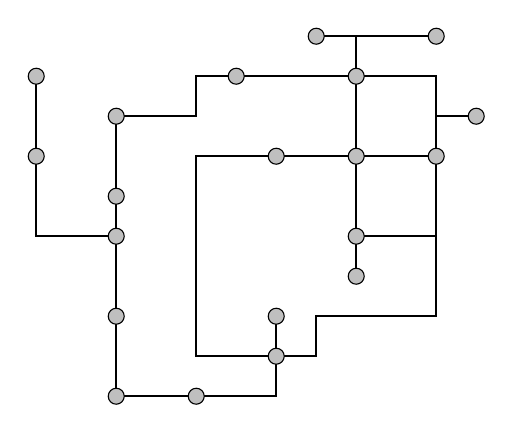
\begin{tikzpicture}[x=0.2in,y=0.2in,every node/.style={circle,fill=lightgray,
                          draw=black,text width=1em,align=center}]
        \draw[thick] (2,0) -- (2,7) -- (4,7) -- (4,8) -- (10,8) --
              (10,2) -- (7,2) -- (7,1) -- (6,1) -- (6,0) -- (2,0);
        \draw[thick] (8,9) -- (8,3);
        \draw[thick] (8,4) -- (10,4);
        \draw[thick] (7,9) -- (10,9);
        \draw[thick] (10,6) -- (4,6) -- (4,1) -- (6,1);
        \draw[thick] (10,7) -- (11,7);
        \draw[thick] (2,4) -- (0,4) -- (0,8);
        \draw[thick] (6,1) -- (6,2);

        \draw[fill=lightgray,draw=black] (2,2) circle (0.2);
        \draw[fill=lightgray,draw=black] (2,4) circle (0.2);
        \draw[fill=lightgray,draw=black] (2,5) circle (0.2);
        \draw[fill=lightgray,draw=black] (2,7) circle (0.2);
        \draw[fill=lightgray,draw=black] (5,8) circle (0.2);
        \draw[fill=lightgray,draw=black] (8,8) circle (0.2);
        \draw[fill=lightgray,draw=black] (10,9) circle (0.2);
        \draw[fill=lightgray,draw=black] (8,4) circle (0.2);
        \draw[fill=lightgray,draw=black] (8,3) circle (0.2);
        \draw[fill=lightgray,draw=black] (10,6) circle (0.2);
        \draw[fill=lightgray,draw=black] (6,6) circle (0.2);
        \draw[fill=lightgray,draw=black] (8,6) circle (0.2);
        \draw[fill=lightgray,draw=black] (6,1) circle (0.2);
        \draw[fill=lightgray,draw=black] (6,2) circle (0.2);
        \draw[fill=lightgray,draw=black] (4,0) circle (0.2);
        \draw[fill=lightgray,draw=black] (2,0) circle (0.2);
        \draw[fill=lightgray,draw=black] (11,7) circle (0.2);
        \draw[fill=lightgray,draw=black] (0,6) circle (0.2);
        \draw[fill=lightgray,draw=black] (0,8) circle (0.2);
        \draw[fill=lightgray,draw=black] (7,9) circle (0.2);
      \end{tikzpicture}
\end{wrapfigure}

Welcome to the world of \textbf{Mobile Monsters}, or \textbf{\mappMobimon}
for short! Not to be confused with the similarly named video game series loved
by fans the world over, \mappMobimon{} is a \textit{completely original} concept
where Trainers befriend monsters and use them to battle opponents. (Cough.)

Under the guidance of your mentor, \textbf{Dr. Treename}, you will soon set off
on your adventure to befriend the \mappMobimon{} of the \textbf{Kantor region}.
You'll meet many strange characters, but if you can solve their problems
they just might lead you to the location of the \textbf{Dojo Masters}.
By earning their respect, you'll be allowed to enter the
\textbf{\mappMobimon{} Tournament} for the chance to be crowned
\textbf{\mappMobimon{} Champion}! Maybe you'll even discover the location
of the Legendary \mappMobimon{} \(\mu\)Too?...

As you might expect, most of the challenges you'll face today won't actually
be combat related. In the world of \mappMobimon{}, nothing is more important
than your \textbf{problem-solving abilities}. So sharpen your minds and
pencils, because you never know when a wild \textbf{puzzle} will appear!


%%% Local Variables:
%%% mode: latex
%%% TeX-master: "../mapp-hsc17-game-book"
%%% End:


\phChapter{Rules}
%!TEX root =../mapp-challenge-18-game-book.tex
% ^ leave for LaTeXTools build functionality

Welcome to the world of \textbf{Mobile Monsters}, or \mappMobimon{} for short!
Not to be confused with a similarly named video game series loved
by fans the world over, \mappMobimon{} is a completely original concept
where Trainers befriend monsters and use them to battle opponents.
(Cough.) Of course,
as your team journeys to become today's \mappMobimon{} Champion,
you should expect a wild \textbf{puzzle} or two to appear...

\phSection{Leagues}

Each team is registered in either the Competitive or Recreational League.
If both Leagues are playing simultaneously today at your campus, then all
scoring and awards are handled separately in both Leagues.

\phSection{Schedule}

The game officially begins at \underline{\hspace{5em}} and ends
four hours later at \underline{\hspace{5em}}. All solutions are due at
Game Control by the end of the game; late submissions will not be considered.

\phSection{Opening Puzzle}

The game begins with an Opening Puzzle to warm things up. Solving this
puzzle quickly will earn your team \textbf{5 Victory Points} and allow
you to immediately move on to the rest of the puzzles!
Don't worry about getting stuck, as all remaining
teams will be allowed to move on
at \underline{\hspace{5em}}. However, you cannot earn Victory Points for
this puzzle after that time.

\phSection{Main Puzzles}

After solving the Opening Puzzle, you will receive four
Main Puzzles. While you'll be given explicit instructions on how to
reveal the word or phrase that solves each Main Puzzle, you'll have to
rely on your mathematical modeling and problem-solving abilities to actually
make it happen. Report your solution to Game Control before the end of
the game, and your team will earn \textbf{15 Victory Points each},
for a maximum total of \textbf{60 Victory Points}.

\newpage

\phSection{Bonus Puzzle}

Along with the four Main Puzzles you will be given a Bonus Puzzle. This
optimization puzzle doesn't have a unique solution, but you should still
attempt to submit the best solution you can to Game Control before the
game ends. That's because if your team is tied in
Victory Points with another team, your scores on the Bonus Puzzle will be used
to \textbf{break the tie}. You may submit up to three solutions throughout
the game (including any invalid submissions), and your best solution of the
three will be considered.

\phSection{Cryptic Puzzles}

You will be given the opportunity to solve an additional Cryptic Puzzle for
every Main Puzzle you solve. These puzzles aren't as straight-forward
as to their solution techniques, but your team might be able to use your
critical thinking to extract a hidden word or phrase. Submitting this
solution to Game Control will earn your team \textbf{5 Victory Points each},
for a maximum total of \textbf{20 Victory Points}.
Teams stuck on a Main Puzzle will get their shot eventually: all
Cryptic Puzzles will become available to all teams at \underline{\hspace{5em}},
one hour before the game ends.

\phSection{Metapuzzle}

If your team is clever enough to solve all four Cryptic Puzzles, a final
Metapuzzle will become available. A correct solution submitted to Game
Control is worth \textbf{10 Victory Points}. This puzzle will become available
to all teams at \underline{\hspace{5em}},
one hour before the game ends.

\phSection{Another Puzzle?}

Shrewd players may discover how to earn an additional
\textbf{5 Victory Points} for their team...

\phSection{Hints}

Recreational teams may ask for hints at Game Control at any time during
the game, for any puzzle. Competitive teams may only ask for hints to help with
the Main Puzzles during the final hour of the game, starting at
\underline{\hspace{5em}}.

\phSection{Winning the Game}

The team that earns the \textbf{most Victory Points out of 100}
by the end of the game is the \textbf{winner}. If any teams are tied,
their Bonus Puzzle scores will be used to break the tie. If that's not enough,
then the tie will be broken based on how quickly those teams earned their
Victory Points (the time each team submitted its last correct puzzle solution).

\newpage

\phSection{Additional Rules}

\begin{itemize}
\item Players should not do anything which
would interfere with other teams solving puzzles. Be a good sport!
\item Teachers and chaperones are not allowed to help Competitive teams solve
puzzles, but they may serve as a means of communication between those teams and
Game Control when appropriate (e.g. for rules clarifications).
\item Teams may use any resources they have brought (phones, computers, etc.)
to solve puzzles, but Competitive Teams may not receive any direct
assistance from outside their team (e.g. you can't Phone a Friend).
\item Players must remain within any physical boundaries set by both
Game Control and their teacher/chaperone at all times.
\item Teachers/chaperones are responsible for their students at
all times.
\item Since this game will be played at different campuses on different
days, please do not spoil any of today's puzzles or solutions online until
the game book is released publicly on MaPPmath.org!
\item Contact Game Control immediately in the case of emergency
or any issues with these rules.
\end{itemize}

%%% Local Variables:
%%% mode: latex
%%% TeX-master: "../mapp-hsc17-game-book"
%%% End:


\phChapter{Code Sheet}
%!TEX root =../mapp-challenge-18-game-book.tex
% ^ leave for LaTeXTools build functionality

\begin{center}\small
  \begin{tabular}{c|c|c|c|c|c|c}
    Letter &
      Decimal &
      Binary &
      Morse Code &
      Braille &
      Pig Pen &
      ROT13\\\hline
    A &
      1 &
      00001 &
      \morseDit\morseDah &
      \braille{a}&
      {\pigpenfont A}&
      N\\
    B &
      2 &
      00010 &
      \morseDah\morseDit\morseDit\morseDit &
      \braille{b}&
      {\pigpenfont B}&
      O\\
    C &
      3 &
      00011 &
      \morseDah\morseDit\morseDah\morseDit &
      \braille{c}&
      {\pigpenfont C}&
      P\\
    D &
      4 &
      00100 &
      \morseDah\morseDit\morseDit &
      \braille{d}&
      {\pigpenfont D}&
      Q\\
    E &
      5 &
      00101 &
      \morseDit &
      \braille{e}&
      {\pigpenfont E}&
      R\\
    F &
      6 &
      00110 &
      \morseDit\morseDit\morseDah\morseDit &
      \braille{f}&
      {\pigpenfont F}&
      S\\
    G &
      7 &
      00111 &
      \morseDah\morseDah\morseDit &
      \braille{g}&
      {\pigpenfont G}&
      T\\
    H &
      8 &
      01000 &
      \morseDit\morseDit\morseDit\morseDit &
      \braille{h}&
      {\pigpenfont H}&
      U\\
    I &
      9 &
      01001 &
      \morseDit\morseDit &
      \braille{i}&
      {\pigpenfont I}&
      V\\
    J &
      10 &
      01010 &
      \morseDit\morseDah\morseDah\morseDah &
      \braille{j}&
      {\pigpenfont J}&
      W\\
    K &
      11 &
      01011 &
      \morseDah\morseDit\morseDah &
      \braille{k}&
      {\pigpenfont K}&
      X\\
    L &
      12 &
      01100 &
      \morseDit\morseDah\morseDit\morseDit &
      \braille{l}&
      {\pigpenfont L}&
      Y\\
    M &
      13 &
      01101 &
      \morseDah\morseDah &
      \braille{m}&
      {\pigpenfont M}&
      Z\\
    N &
      14 &
      01110 &
      \morseDah\morseDit &
      \braille{n}&
      {\pigpenfont N}&
      A\\
    O &
      15 &
      01111 &
      \morseDah\morseDah\morseDah &
      \braille{o}&
      {\pigpenfont O}&
      B\\
    P &
      16 &
      10000 &
      \morseDit\morseDah\morseDah\morseDit &
      \braille{p}&
      {\pigpenfont P}&
      C\\
    Q &
      17 &
      10001 &
      \morseDah\morseDah\morseDit\morseDah &
      \braille{q}&
      {\pigpenfont Q}&
      D\\
    R &
      18 &
      10010 &
      \morseDit\morseDah\morseDit &
      \braille{r}&
      {\pigpenfont R}&
      E\\
    S &
      19 &
      10011 &
      \morseDit\morseDit\morseDit &
      \braille{s}&
      {\pigpenfont S}&
      F\\
    T &
      20 &
      10100 &
      \morseDah &
      \braille{t}&
      {\pigpenfont T}&
      G\\
    U &
      21 &
      10101 &
      \morseDit\morseDit\morseDah &
      \braille{u}&
      {\pigpenfont U}&
      H\\
    V &
      22 &
      10110 &
      \morseDit\morseDit\morseDit\morseDah &
      \braille{v}&
      {\pigpenfont V}&
      I\\
    W &
      23 &
      10111 &
      \morseDit\morseDah\morseDah &
      \braille{w}&
      {\pigpenfont W}&
      J\\
    X &
      24 &
      11000 &
      \morseDah\morseDit\morseDit\morseDah &
      \braille{x}&
      {\pigpenfont X}&
      K\\
    Y &
      25 &
      11001 &
      \morseDah\morseDit\morseDah\morseDah &
      \braille{y}&
      {\pigpenfont Y}&
      L\\
    Z &
      26 &
      11010 &
      \morseDah\morseDah\morseDit\morseDit &
      \braille{z}&
      {\pigpenfont Z}&
      M\\
  \end{tabular}
\end{center}

\normalsize

%%% Local Variables:
%%% mode: latex
%%% TeX-master: "../mapp-hsc17-game-book"
%%% End:



\phChapter{Scoresheet}
%!TEX root =../mapp-hsc17-game-book.tex
% ^ leave for LaTeXTools build functionality


{\small Game Control and your team each have a copy of this scoresheet.
When submitting solutions, bring your team's copy to Game Control
to be updated.}

\vfill

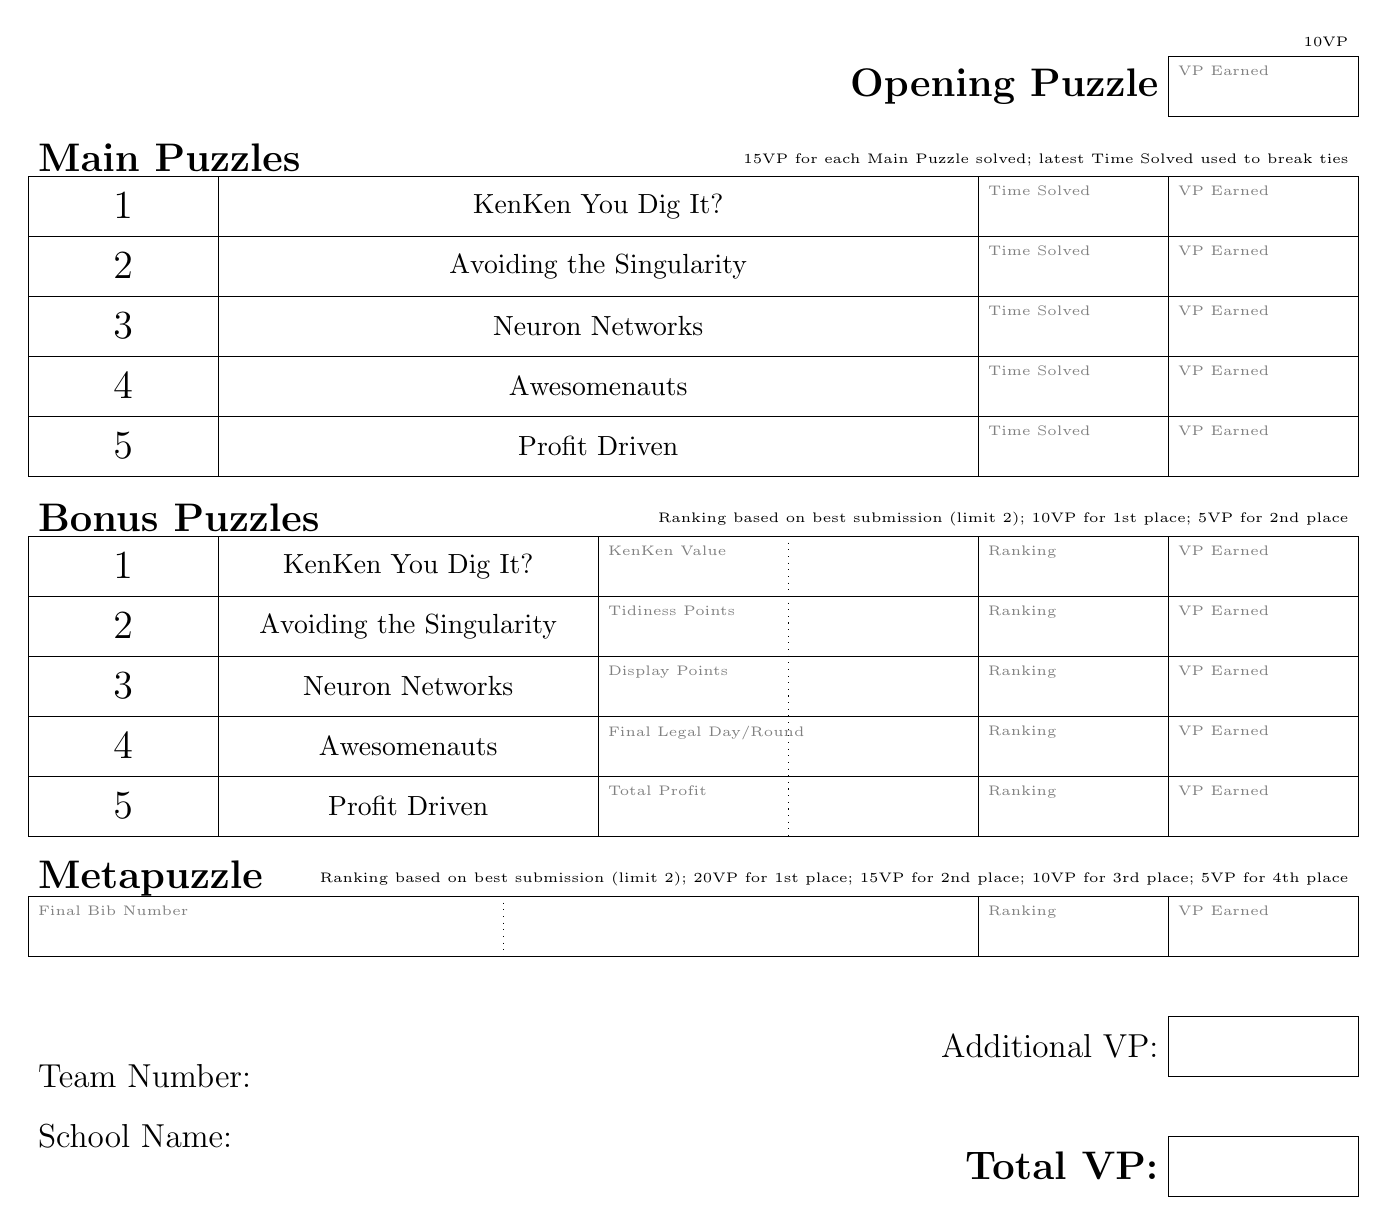
\begin{tikzpicture}[x=0.95in,y=-0.3in]
  % \draw (0,0) rectangle +(6,1);
  % \draw (1,0) -- +(0,1);

  \node[anchor=east] at (6,2.5) {\Large\bf Opening Puzzle};
  \draw (6,2) rectangle +(1,1);
  % \draw (5,2) -- +(0,1);
  % % \draw (6,2) -- +(0,1);
  % \node[color=gray,anchor=north west] at (0,2)
  %   {\tiny Time Submitted};
  % \node[color=gray,anchor=north west] at (5,2)
  %   {\tiny Time Submitted};
  \node[color=gray,anchor=north west] at (6,2)
    {\tiny VP Earned};
  \node[anchor=south east] at (7,2)
    {\tiny 10VP};

  \node[anchor=west] at (0,3.7) {\Large\bf Main Puzzles};
  \draw (0,4) rectangle +(7,5);
  \draw (0,5) -- +(7,0);
  \draw (0,6) -- +(7,0);
  \draw (0,7) -- +(7,0);
  \draw (0,8) -- +(7,0);
  \draw (1,4) -- +(0,5);
  \draw (5,4) -- +(0,5);
  \draw (6,4) -- +(0,5);
  \node at (0.5,4.5) {\Large 1};
  \node at (0.5,5.5) {\Large 2};
  \node at (0.5,6.5) {\Large 3};
  \node at (0.5,7.5) {\Large 4};
  \node at (0.5,8.5) {\Large 5};
  \node at (3,4.5) {KenKen You Dig It?};
  \node at (3,5.5) {Avoiding the Singularity};
  \node at (3,6.5) {Neuron Networks};
  \node at (3,7.5) {Awesomenauts};
  \node at (3,8.5) {Profit Driven};
  \node[color=gray,anchor=north west] at (5,4)
    {\tiny Time Solved};
  \node[color=gray,anchor=north west] at (5,5)
    {\tiny Time Solved};
  \node[color=gray,anchor=north west] at (5,6)
    {\tiny Time Solved};
  \node[color=gray,anchor=north west] at (5,7)
    {\tiny Time Solved};
  \node[color=gray,anchor=north west] at (5,8)
    {\tiny Time Solved};
  \node[color=gray,anchor=north west] at (6,4)
    {\tiny VP Earned};
  \node[color=gray,anchor=north west] at (6,5)
    {\tiny VP Earned};
  \node[color=gray,anchor=north west] at (6,6)
    {\tiny VP Earned};
  \node[color=gray,anchor=north west] at (6,7)
    {\tiny VP Earned};
  \node[color=gray,anchor=north west] at (6,8)
    {\tiny VP Earned};
  \node[anchor=south east] at (7,4)
    {\tiny 15VP for each Main Puzzle solved; latest Time Solved used to break ties};

  \node[anchor=west] at (0,9.7) {\Large\bf Bonus Puzzles};
  \draw (0,10) rectangle +(7,5);
  \draw (0,11) -- +(7,0);
  \draw (0,12) -- +(7,0);
  \draw (0,13) -- +(7,0);
  \draw (0,14) -- +(7,0);
  \draw (1,10) -- +(0,5);
  \draw (3,10) -- +(0,5);
  \draw[dotted] (4,10) -- +(0,5);
  \draw (5,10) -- +(0,5);
  \draw (6,10) -- +(0,5);
  \node at (0.5,10.5) {\Large 1};
  \node at (0.5,11.5) {\Large 2};
  \node at (0.5,12.5) {\Large 3};
  \node at (0.5,13.5) {\Large 4};
  \node at (0.5,14.5) {\Large 5};
  \node at (2,10.5) {KenKen You Dig It?};
  \node at (2,11.5) {Avoiding the Singularity};
  \node at (2,12.5) {Neuron Networks};
  \node at (2,13.5) {Awesomenauts};
  \node at (2,14.5) {Profit Driven};
  \node[color=gray,anchor=north west] at (3,10)
    {\tiny KenKen Value};
  \node[color=gray,anchor=north west] at (3,11)
    {\tiny Tidiness Points};
  \node[color=gray,anchor=north west] at (3,12)
    {\tiny Display Points};
  \node[color=gray,anchor=north west] at (3,13)
    {\tiny Final Legal Day/Round};
  \node[color=gray,anchor=north west] at (3,14)
    {\tiny Total Profit};
  \node[color=gray,anchor=north west] at (5,10)
    {\tiny Ranking};
  \node[color=gray,anchor=north west] at (5,11)
    {\tiny Ranking};
  \node[color=gray,anchor=north west] at (5,12)
    {\tiny Ranking};
  \node[color=gray,anchor=north west] at (5,13)
    {\tiny Ranking};
  \node[color=gray,anchor=north west] at (5,14)
    {\tiny Ranking};
  \node[color=gray,anchor=north west] at (6,10)
    {\tiny VP Earned};
  \node[color=gray,anchor=north west] at (6,11)
    {\tiny VP Earned};
  \node[color=gray,anchor=north west] at (6,12)
    {\tiny VP Earned};
  \node[color=gray,anchor=north west] at (6,13)
    {\tiny VP Earned};
  \node[color=gray,anchor=north west] at (6,14)
    {\tiny VP Earned};
  \node[anchor=south east] at (7,10)
    {\tiny Ranking based on best submission (limit 2); 10VP for 1st place;
      5VP for 2nd place};

  \node[anchor=west] at (0,15.7) {\Large\bf Metapuzzle};
  \draw (0,16) rectangle +(7,1);
  \draw[dotted] (2.5,16) -- +(0,1);
  \draw (5,16) -- +(0,1);
  \draw (6,16) -- +(0,1);
  \node[color=gray,anchor=north west] at (0,16)
    {\tiny Final Bib Number};
  \node[color=gray,anchor=north west] at (5,16)
    {\tiny Ranking};
  \node[color=gray,anchor=north west] at (6,16)
    {\tiny VP Earned};
  \node[anchor=south east] at (7,16)
    {\tiny Ranking based on best submission (limit 2); 20VP for 1st place;
      15VP for 2nd place; 10VP for 3rd place; 5VP for 4th place};

  % \draw[dotted] (0,18) rectangle +(3,1);
  % \draw[dotted] (2,18) -- +(0,1);

  \node[anchor=west] at (0,19) {\large Team Number:};
  \node[anchor=west] at (0,20) {\large School Name:};

  \node[anchor=east] at (6,18.5) {\large Additional VP:};
  \draw (6,18) rectangle +(1,1);

  \node[anchor=east] at (6,20.5) {\Large\bf Total VP:};
  \draw (6,20) rectangle +(1,1);
\end{tikzpicture}

\vfill
\vfill
%
% \vspace{1em}
%
% {\noindent\LARGE Team Number: \underline{\hspace{0.5in}}
% School Name: \underline{\hspace{3in}}}


%%% Local Variables:
%%% mode: latex
%%% TeX-master: "../mapp-hsc17-game-book"
%%% End:


\phChapter{Campus Guidelines}
%!TEX root =../mapp-challenge-18-game-book.tex
% ^ leave for LaTeXTools build functionality

Here are some guidelines for local campuses on how to prepare for and
run the event.

\phSection{Schedule Template}

\begin{itemize}
  \item 0:00 - Registration
  \item 0:45 - Orientation
  \item 1:00 - Game Begins with Opening Puzzle
  \item 2:00 - Opening Puzzle due
  \item 4:00 - Cryptic/Meta Puzzles released
  \item 5:00 - Game Ends (all solutions due)
  \item 5:30 - Wrap-Up and Awards
  \item 6:00 - Dismissal
\end{itemize}

\phSection{Classroom Space}

A large \textbf{lecture hall} is recommended for running Registration,
Orientation, and the Wrap-Up. Game Control can be stationed there during
the game as well.

Each team should be given a separate \textbf{classroom} so that they may
openly collaborate with teammates without spoiling puzzles for other teams.
It is useful to affix \textbf{printed signs} on each classroom and Game
Control to help players navigate your space, as well as any additional
signage required to get around. \textbf{Blank templates with the MaPP logo}
are available in the Appendix.

\phSection{Team Supplies}

\textbf{Scissors and tape} should be provided in each classroom.
In addition, \textbf{chalk or whiteboard markers} should be provided if
teams will have access to chalkboards or whiteboards in their room.
We recommend \textbf{inviting teams to bring additional supplies}, such as
graph paper, colored pencils, and simple calculators.

Note that teams may also choose to bring smartphones, laptops, cameras,
and so on. Due to the wide availability of such technology (particularly
phones), we discourage campuses from banning outside equipment, but also
do not suggest to explicitly recommend such items as they aren't required
to enjoy or be competitive in this game. The puzzles are
designed so that they cannot be solved using Google or brute force methods,
with one exception. Savvy programmers might be able to write code to
help optimize their team's Bonus Puzzle solutions, which is why the Bonus
Puzzle is only used to break ties.

\phSection{Copies}

All puzzles are designed to be printed/copied in \textbf{grayscale}, both
for the convience of campuses and for accessibility by players.
See below to account for how many copies are needed throughout the game.
It is recommended to print copies for at least
\textbf{two more teams than you expect to participate} as extras, depending
on your access to last-minute copying.

\textbf{Each volunteer} working at \textbf{Game Control} should have a
\textbf{complete copy of the game book in a binder} for their reference.

\phSection{Registration}

\textbf{Each player} should receive a \textbf{packet} containing the
\textbf{Story}, \textbf{Rules}, and \textbf{Code Sheet} pages of the game book.
They should also receive
a \textbf{pencil} and \textbf{notepad} for use during the Opening Puzzle
and the rest of the game.

Some campuses also choose to distribute other giveaways/swag/brochures
at registration. Many bookstores are willing to provide branded disposable
bags to help distribute materials.

Teams should be directed to their assigned classroom where they can
drop off everything except the provided packet, pencil, and notepad.
They should then return to Game Control's lecture hall to await Orientation.

\phSection{Orientation}

The Story and Rules should be reviewed, and any questions from players
should be answered. In particular, boundaries for where players are allowed
to travel during the game should be established.

\phSection{Opening Puzzle}

\textbf{Each team} should receive \textbf{four copies} of the
\textbf{Opening Puzzle} and supporting documents. The deadline for
completing the Opening Puzzle should be clearly communicated.

If you wish for players to \textbf{explore your campus}, then you should
also provide a \textbf{Campus Map} with twenty locations labeled \(1\)-\(20\).
The Opening Puzzle solves to four of those numbers, so players should be
instructed to visit those four locations. For larger destinations, you should
specify where to visit (e.g. the front door). You may choose to either place
a \textbf{volunteer} at each location to distribute a token to each team that
successfully finds it, or an \textbf{envelope} of tokens for teams to claim at
each location. You may choose to have teams pick up a copy of one of the four
\textbf{Main Puzzles} at each location to serve as this token, but these should
not be the only copies of the Main Puzzles given to each team (see below).

Once this puzzle has been reviewed for all players, you may dismiss the players
to begin solving. Once each team completes the puzzle, they should present
their solution and/or tokens to Game Control. In return they should receive
an \textbf{envelope} containing \textbf{four copies each} of
\textbf{Main Puzzles 1-4} and the \textbf{Bonus Puzzle}, including supporting
documents. They should also
receive a \textbf{Scoresheet} to mirror the \textbf{Scoresheet copy} maintained
at Game Control, updated with the results of the Opening Puzzle.

At the deadline for the puzzle, all remaining teams should return to
Game Control to pick up their puzzle envelope and scoresheet, and move
on to the Main/Bonus Puzzles. If additional
volunteers have been organized to facilitate the exploration of campus,
you may choose to dismiss them at this time.

\phSection{Post-Opening Gameplay}

After the Opening Puzzle,
teams can remain in their provided classroom for the duration of the
competition, except to submit solutions to Game Control.

A volunteer should stand at the door of Game Control to ensure at most
one team is allowed in Game Control at all times. Solutions to the
Main Puzzles, Cryptic Puzzles, and the Metapuzzle are all short words/phrases
and may be communicated to Game Control verbally, but may be written out
on paper if clarification is required. The solution to the Hidden Puzzle
is also a short word/phrase and may be communicated verbally or written out,
but Game Control should only confirm the existence of the Hidden Puzzle
explicitly after receiving a correct solution. Players should be asked
which puzzle they are attempting to solve before giving a solution.

As each Main Puzzle is solved, that team should receive a \textbf{packet}
containing \textbf{four copies} of the corresponding \textbf{Cryptic Puzzle},
including supporting documents.
Once each team has solved all four Cryptic Puzzles, they should receive a
\textbf{packet} containing \textbf{four copies} of the \textbf{Metapuzzle},
including supporting documents.
All teams are allowed to pick up an \textbf{envelope} containing all
unclaimed copies of the Cryptic Puzzles and Metapuzzle during the final hour
of the game.

Each time a puzzle is correctly solved, it should be updated by Game Control
on both their copy and the team's copy of the Scoresheet, including a
timestamp.

Recreational teams are allowed to ask for hints at Game Control at any time
for any Main Puzzle, Cryptic Puzzle, or Metapuzzle. Game Control should ask
players to explain the work they've
done thus far, and give a single hint that should help the team make some
amount of progress. Different teams may receive different hints for the same
puzzle depending on their progress.

Competitive teams may receive hints for the Main Puzzles during the final
hour of the game. Game Control should provide as much help as is necessary;
the goal of the Main Puzzles is to expose players to new types of mathematics,
so most teams should solve most of the Main Puzzles by the end of the game.

Teams cannot be given hints for the Bonus Puzzle or Hidden Puzzle.

Each team is allowed three submissions of the Bonus Puzzle. Generally this
puzzle should be judged by Game Control in front of the players to confirm
the validity of the submission. Each submission is recorded on both
Scoresheets, including crossing out a box for an invalid submission.
Only the best submission from each team is used. If the game has ended
with multiple teams in line for Game Control, all submissions for all teams
should be collected as quickly as possible and graded. Teams may not submit
multiple Bonus Puzzle solutions after the game has ended.

\phSection{Food}

Campuses that will be running the event through lunchtime are encouraged to
provide a \textbf{pizza lunch} for players. This lunch should not interrupt the
game; rather, players should be able to grab a bite to eat to have while they
continue to solve puzzles. In addition, \textbf{snacks}
(fruit, granola bars, etc.) and \textbf{drinks} (bottled water) are nice for
players to have access to during the game. Don't forget to provide
appropriate \textbf{plates, cutlery, napkins, and trashbags}.

This food can be distributed at a \textbf{central location near Game Control}
(but not inside Game Control's room).

\phSection{Wrap-Up and Awards}

At the end of the game, teams should straighten up their classrooms before
returning to Game Control for the Wrap-Up. \textbf{Trash bags} may be
provided for this purpose.

Teams should line up outside Game Control until results have been tabulated.
Once all results have been determined, teams may be seated inside Game Control.
\textbf{Solutions} to all puzzles should be projected and reviewed with
all players.

Awards for Recreational/Competitive teams are treated completely separately
if both Leagues are present.
\textbf{Certificates} should be distributed in random order to all teams placing
below 3rd place. A \textbf{3rd Place Certificate/Trophy} is then awarded.
After reminding the 1st place team to be respectful, a
\textbf{2nd Place Certificate/Trophy} is then awarded, followed by the
\textbf{1st Place Certificate/Trophy}. Opportunities for photographs should
be allowed during this process and after dismissal.

After awards are done, teams may be dismissed.

\phSection{Shirts/Theming}

Campuses may choose to provide/sell \textbf{shirts} to volunteers and players,
keeping in mind that volunteers should be identifyable to players by sight.
To this end, we encourage distributing shirts at Wrap-Up, or using different
colors for players/volunteers.

Optionally, you may encourage teams and/or volunteers to
wear school colors/shirts, or to develop a team name/theme fitting the
game's theme.

\phSection{Social Media}

Players/teachers/volunteers should be encouraged to tag \texttt{@MaPPmath}
and \texttt{\#\phEventAbbr} on Twitter with non-spoiler posts/media during
and after the event.

\phSection{ClueKeeper}

The \textbf{ClueKeeper} app will be piloted at select campuses for this
event. All rule changes relevant to the usage of ClueKeeper's
solution submissions and GPS enforcement should be made clear to players
via the app. Each team must have access to an iOS or Android
\textbf{smart device} with the game downloaded to participate, which
may be provided by your campus or the participating teams.
ClueKeeper may be downloaded from \texttt{cluekeeper.com}. A helpful
\textbf{ClueKeeper FAQ} is available in the appendix to support your players.

%%% Local Variables:
%%% mode: latex
%%% TeX-master: t
%%% End:




%opening puzzle
\phPart{Opening Puzzle}
%!TEX root =../mapp-challenge-18-game-book.tex
% ^ leave for LaTeXTools build functionality

\phChapterWorksheet{The Kantor Region}{Opening Puzzle}



\begin{center}
  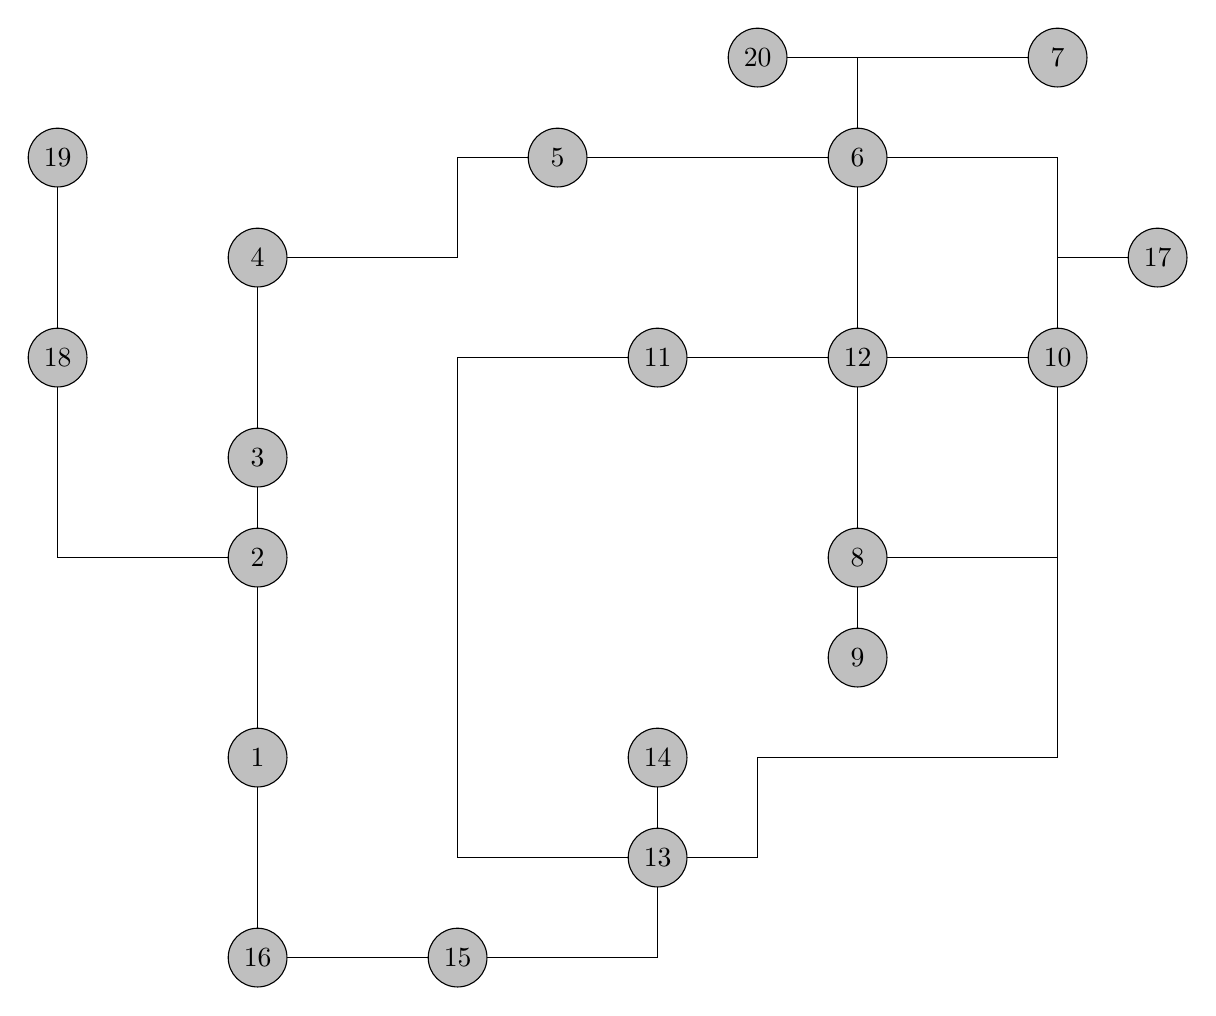
\begin{tikzpicture}[x=0.5in,y=0.5in,every node/.style={circle,fill=lightgray,draw=black,text width=1em,align=center}]
    \draw (2,0) -- (2,7) -- (4,7) -- (4,8) -- (10,8) --
          (10,2) -- (7,2) -- (7,1) -- (6,1) -- (6,0) -- (2,0);
    \draw (8,9) -- (8,3);
    \draw (8,4) -- (10,4);
    \draw (7,9) -- (10,9);
    \draw (10,6) -- (4,6) -- (4,1) -- (6,1);
    \draw (10,7) -- (11,7);
    \draw (2,4) -- (0,4) -- (0,8);
    \draw (6,1) -- (6,2);

    \node at (2,2) {1};
    \node at (2,4) {2};
    \node at (2,5) {3};
    \node at (2,7) {4};
    \node at (5,8) {5};
    \node at (8,8) {6};
    \node at (10,9) {7};
    \node at (8,4) {8};
    \node at (8,3) {9};
    \node at (10,6) {10};
    \node at (6,6) {11};
    \node at (8,6) {12};
    \node at (6,1) {13};
    \node at (6,2) {14};
    \node at (4,0) {15};
    \node at (2,0) {16};
    \node at (11,7) {17};
    \node at (0,6) {18};
    \node at (0,8) {19};
    \node at (7,9) {20};
  \end{tikzpicture}
\end{center}

% Include below for aucTeX integration
%%% Local Variables:
%%% mode: latex
%%% TeX-master: "../mapp-challenge-18-game-book"
%%% End:


% %main puzzles
\phPart{Main Puzzles}
%!TEX root =../mapp-challenge-18-game-book.tex
% ^ leave for LaTeXTools build functionality

\phChapterWorksheet{Go Get 'Em!}{Main Puzzle 3}

While catching \mappMobimon{} on Interstate \(\sqrt{1.73205...}\),
you run across a wise old
\mappMobimon{} trainer who challenges you to a \mappMobimon{} battle. But not
just any \mappMobimon{} battle! This is a \textbf{puzzle battle.} The reward?
The location where all the \mappMobimon{} gather.

The old man tells you about a game he enjoyed in his youth called \textbf{Go.}

Go is a game of strategy played with black and white pieces on a grid. It's a
bit like chess, except instead of lots of kinds of pieces, each player only has
\textbf{one kind of piece, the stone.} And instead of playing on the squares,
players play on the \textbf{intersections of the grid lines,} and you can play
on board going from 9 by 9 up to 19 by 19. And \textbf{black goes first.} Maybe
it's not all that much like chess.

Much like chess, though, part of the strategy relies on \textbf{capturing your
  opponent's stones.} To capture you have to know about stones, groups of
stones, and their \textbf{liberties.}

Stones typically don't stay isolated for very long from other stones of the same
color. Stones form a \textbf{group} if they are \textbf{directly next to each
  other on the grid,} but \textbf{not diagonally.}

These stones form a group.

\begin{center}
  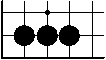
\includegraphics{gogetem/assets/explanation1-crop}
\end{center}

These stones \textbf{do not.} These are just three individual stones.

\begin{center}
  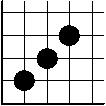
\includegraphics{gogetem/assets/explanation2-crop}
\end{center}

An individual stone has \textbf{liberties.} Liberties are the \textbf{empty
  spaces directly next to the stone on the grid,} but \textbf{not diagonally.}
So a stone may have \textbf{as many as 4} liberties. If an individual stone has
no liberties, \textbf{it is captured.}

The liberties of the black stones are marked with x's:

\begin{center}
  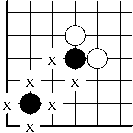
\includegraphics{gogetem/assets/explanation3-crop}
\end{center}

So the black stone on the lower left has \textbf{4 liberties,} and the black
stone on the upper right \textbf{only has two liberties} because the other two
spaces around it are occupied by white stones.

\textbf{Groups of stones share liberties.} A whole group of stones can be
captured at the same time if the whole group has no liberties. The group of
black stones below has \textbf{7 liberties.}

\begin{center}
  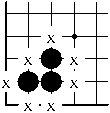
\includegraphics{gogetem/assets/explanation4-crop}
\end{center}

A stone can normally \textbf{not} be played in a space where it has no
liberties, with \textbf{one important exception.} A stone can be placed into a
space where it would have no liberties only if doing so \textbf{captures one or
  more enemy stones.}

The old man lays out several boards in an intermediate size, then says, ``In
each of the Go boards below, there is exactly one stone you can play, white or
black, that will allow you to make a capture. You need to figure out
\textbf{what color stone} to play and \textbf{where to play it} in order to make
a capture. Do that, and you will already know where all the \mappMobimon{}
gather.''

You notice that each of the boards the old man shows you is \textbf{13 by
  13.} There are also \textbf{26 letters in the alphabet.} Hmmm...

\begin{center}
  \contournumber{64}
  \begin{tikzpicture}
    \node[anchor=south west,inner sep=0] (image) at
    (0,0){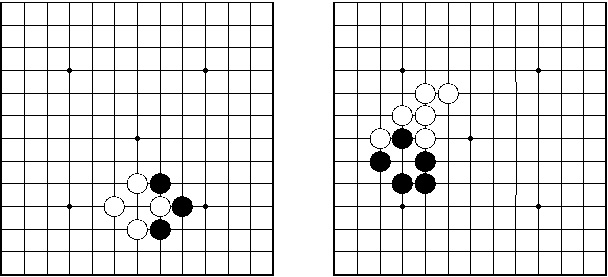
\includegraphics[scale=1.5]{gogetem/assets/boards1-crop}};
    % left board coordinate system
    \foreach \x in {0,...,12}
    \node at (\x * 0.58, 7.3){\contour{black}{\AlphAlph{\x + 14}}};
    \foreach \x in {0,...,12}
    \node at (-0.25, \x * 0.58){\contour{black}{\textcolor{white}{\AlphAlph{13 -
          \x}}}};
    % right board coordinate system
  \foreach \x in {0,...,12} \node at (8.5 + \x * 0.58,
  7.3){\contour{black}{\AlphAlph{\x + 14}}}; \foreach \x in {0,...,12} \node at
  (8.2, \x * 0.58){\contour{black}{\textcolor{white}{\AlphAlph{13 - \x}}}};
  \end{tikzpicture}

  \begin{tikzpicture}
    \node[anchor=south west,inner sep=0] (image) at
    (0,0){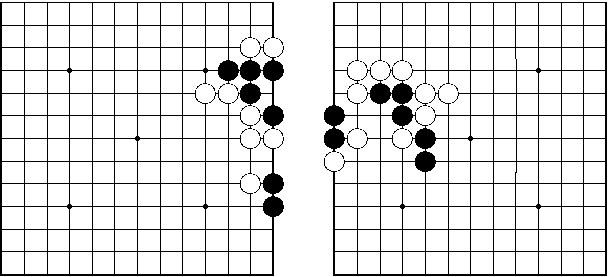
\includegraphics[scale=1.5]{gogetem/assets/boards2-crop}};
    % left board coordinate system
    \foreach \x in {0,...,12}
    \node at (\x * 0.58, 7.3){\contour{black}{\AlphAlph{\x + 14}}};
    \foreach \x in {0,...,12}
    \node at (-0.25, \x * 0.58){\contour{black}{\textcolor{white}{\AlphAlph{13 -
          \x}}}};
    % right board coordinate system
    \foreach \x in {0,...,12}
    \node at (8.5 + \x * 0.58, 7.3){\contour{black}{\AlphAlph{\x + 14}}};
    \foreach \x in {0,...,12}
    \node at (8, \x * 0.58){\contour{black}{\textcolor{white}{\AlphAlph{13 - \x}}}};
  \end{tikzpicture}

  \begin{tikzpicture}
    \node[anchor=south west,inner sep=0] (image) at
    (0,0){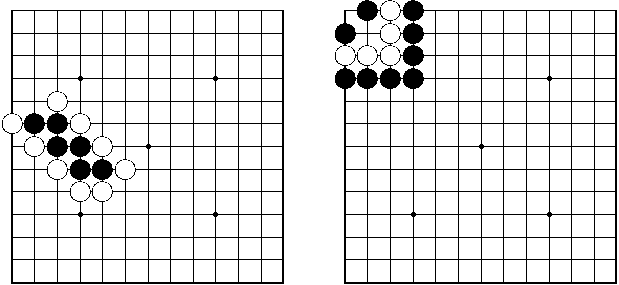
\includegraphics[scale=1.5]{gogetem/assets/boards3-crop}};
    % left board coordinate system
    \foreach \x in {0,...,12}
    \node at (\x * 0.58, 7.3){\contour{black}{\AlphAlph{\x + 14}}};
    \foreach \x in {0,...,12}
    \node at (-0.25, \x * 0.58){\contour{black}{\textcolor{white}{\AlphAlph{13 -
          \x}}}};
    % right board coordinate system
    \foreach \x in {0,...,12}
    \node at (8.7 + \x * 0.58, 7.5){\contour{black}{\AlphAlph{\x + 14}}};
    \foreach \x in {0,...,12}
    \node at (8.2, \x * 0.58){\contour{black}{\textcolor{white}{\AlphAlph{13 - \x}}}};
  \end{tikzpicture}

  \begin{tikzpicture}
    \node[anchor=south west,inner sep=0] (image) at
    (0,0){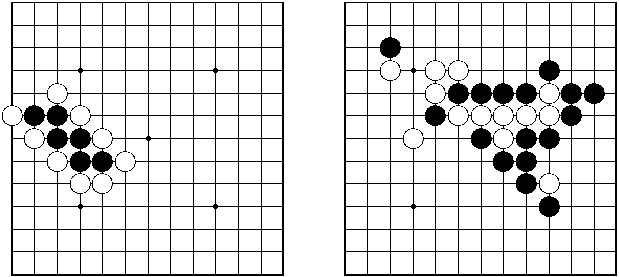
\includegraphics[scale=1.5]{gogetem/assets/boards4-crop}};
    % left board coordinate system
    \foreach \x in {0,...,12}
    \node at (0.3 + \x * 0.58, 7.5){\contour{black}{\AlphAlph{\x + 14}}};
    \foreach \x in {0,...,12}
    \node at (-0.25, \x * 0.58){\contour{black}{\textcolor{white}{\AlphAlph{13 -
          \x}}}};
    % right board coordinate system
    \foreach \x in {0,...,12}
    \node at (8.7 + \x * 0.58, 7.3){\contour{black}{\AlphAlph{\x + 14}}};
    \foreach \x in {0,...,12}
    \node at (8.2, \x * 0.58){\contour{black}{\textcolor{white}{\AlphAlph{13 - \x}}}};
  \end{tikzpicture}

  \begin{tikzpicture}
    \node[anchor=south west,inner sep=0] (image) at
    (0,0){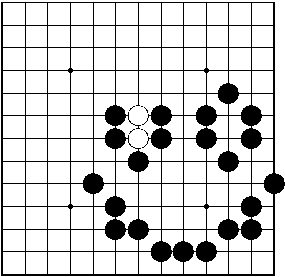
\includegraphics[scale=1.5]{gogetem/assets/boards5-crop}};
    % left board coordinate system
    \foreach \x in {0,...,12}
    \node at (\x * 0.58, 7.3){\contour{black}{\AlphAlph{\x + 14}}};
    \foreach \x in {0,...,12}
    \node at (-0.25, \x * 0.58){\contour{black}{\textcolor{white}{\AlphAlph{13 -
          \x}}}};
  \end{tikzpicture}

\end{center}
Where should you find the \mappMobimon{}?

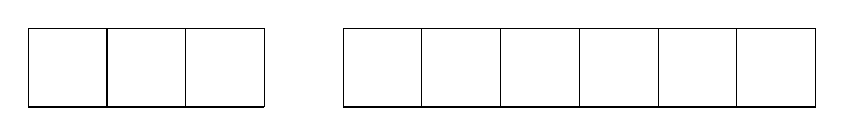
\begin{tikzpicture}
  \draw (0,0) grid (3,1);
  \draw (4,0) grid (10,1);
\end{tikzpicture}

% Include below for aucTeX integration
%%% Local Variables:
%%% mode: latex
%%% TeX-master: "../mapp-challenge-18-game-book"
%%% End:

%!TEX root =../mapp-challenge-18-game-book.tex
% ^ leave for LaTeXTools build functionality

\phChapterWorksheet{When Push Comes to Shove}{Main Puzzle 2}

\newcommand{\mappBoxRow}[2]{
  \fill[color=lightgray] #1 rectangle #2;
  \draw[step=1]          #1 grid #2;
}

% http://oeis.org/A000041 number of partitions
% http://oeis.org/A000009 number of odd/distinct partitions

While training your \mappMobimon{} on Interstate \(i\), you are approached
by \textbf{Dockworker Dave}, who challenges you to a \mappMobimon{} battle!
Of course you accepted... turning him down would be \textbf{rude},
don't you think?

It was a close match, but you win! As Dave gives you your victory money, he
tells you about a group of \textbf{Tattarat} \mappMobimon{} that infest the
warehouse he works in. These obnoxious critters like to
\textbf{rearrange the boxes} in his warehouse, so Dave cuts you a deal.
He'll let you catch a Tattarat for your team, but only if you help
him reorganize his boxes.

The boxes in the warehouse must be \textbf{stacked} so that
each row of boxes is always pressed up against the \textbf{left wall} of the
warehouse, and each row of boxes must have the \textbf{same or less boxes} than
every lower row.

Other than that, it's up to you. For example, there are \textbf{seven}
different ways to stack \textbf{five} boxes.

\begin{center}
  \begin{tikzpicture}[x=0.15in,y=0.15in]
    \mappBoxRow{(0,0)}{(5,1)}

    \draw[thick] (0,0) -- (0, 5);
    \draw[thick] (0,0) -- (5, 0);
  \end{tikzpicture}
  \begin{tikzpicture}[x=0.15in,y=0.15in]
    \mappBoxRow{(0,0)}{(4,1)}
    \mappBoxRow{(0,1)}{(1,2)}

    \draw[thick] (0,0) -- (0, 5);
    \draw[thick] (0,0) -- (5, 0);
  \end{tikzpicture}
  \begin{tikzpicture}[x=0.15in,y=0.15in]
    \mappBoxRow{(0,0)}{(3,1)}
    \mappBoxRow{(0,1)}{(2,2)}

    \draw[thick] (0,0) -- (0, 5);
    \draw[thick] (0,0) -- (5, 0);
  \end{tikzpicture}
  \begin{tikzpicture}[x=0.15in,y=0.15in]
    \mappBoxRow{(0,0)}{(3,1)}
    \mappBoxRow{(0,1)}{(1,2)}
    \mappBoxRow{(0,2)}{(1,3)}

    \draw[thick] (0,0) -- (0, 5);
    \draw[thick] (0,0) -- (5, 0);
  \end{tikzpicture}
  \begin{tikzpicture}[x=0.15in,y=0.15in]
    \mappBoxRow{(0,0)}{(2,1)}
    \mappBoxRow{(0,1)}{(2,2)}
    \mappBoxRow{(0,2)}{(1,3)}

    \draw[thick] (0,0) -- (0, 5);
    \draw[thick] (0,0) -- (5, 0);
  \end{tikzpicture}
  \begin{tikzpicture}[x=0.15in,y=0.15in]
    \mappBoxRow{(0,0)}{(2,1)}
    \mappBoxRow{(0,1)}{(1,2)}
    \mappBoxRow{(0,2)}{(1,3)}
    \mappBoxRow{(0,3)}{(1,4)}

    \draw[thick] (0,0) -- (0, 5);
    \draw[thick] (0,0) -- (5, 0);
  \end{tikzpicture}
  \begin{tikzpicture}[x=0.15in,y=0.15in]
    \mappBoxRow{(0,0)}{(1,1)}
    \mappBoxRow{(0,1)}{(1,2)}
    \mappBoxRow{(0,2)}{(1,3)}
    \mappBoxRow{(0,3)}{(1,4)}
    \mappBoxRow{(0,4)}{(1,5)}

    \draw[thick] (0,0) -- (0, 5);
    \draw[thick] (0,0) -- (5, 0);
  \end{tikzpicture}
\end{center}

The dockworker notices your good work.
``Hey, didya say you were aiming to become one of them \mappMobimon{}
Champions? Maybe you're smart enough to solve this \textbf{puzzle} for me
then.'' It seems that if you can count the following different combinations
of stacked boxes, you'll be able to reveal a \textbf{hidden message} by
converting the numbers to appropriate letters (A=1, B=2, and so on).

\begin{multicols}{2}
  \begin{itemize}
    \item %M=13
      The number of ways you can stack either \(2\) or \(6\) boxes.
    \item %O=15
      The number of ways you can stack \(12\) boxes, if every row must
      contain an odd number.
    \item %U=21
      The number of ways you can stack \(8\) boxes, if every row must contain
      less than eight.
    \item %S=19
      The number of ways you can stack up to \(5\) boxes. (An empty room
      counts as one way...)
    \item %E=5
      The number of ways you can stack \(4\) boxes.
  \end{itemize}
\columnbreak
  \begin{itemize}
    \item %T=20
      The number of ways you can stack \(8\) boxes, if every row must contain
      less than seven.
    \item %R=18
      The number of ways you can stack \(13\) boxes, if every row must have
      less boxes than the row below it.
    \item %A=1
      The number of ways you can stack \(42\) boxes, if you can only use one
      row.
    \item %P=16
      The number of ways you can stack \(1\) or \(12\) boxes, if every row must
      have a unique number of boxes.
  \end{itemize}
\end{multicols}


%%SOLUTION%%%
% MOUSETRAP %
%%%%%%%%%%%%%


% Old unused text:

% For example, this configuration looks solid.
% \begin{center}
%   \begin{tikzpicture}
%     \fill[color=lightgray] (0,0) rectangle (4,1);
%     \draw             (0,0) grid (4,1);
%     \fill[color=lightgray] (0,1) rectangle (3,2);
%     \draw             (0,1) grid (3,2);
%     \fill[color=lightgray] (0,2) rectangle (1,3);
%     \draw             (0,2) grid (1,3);
%
%     \draw[thick] (0,0) -- (0, 4);
%     \draw[thick] (0,0) -- (5, 0);
%   \end{tikzpicture}
% \end{center}
%
% But this one isn't so great.
% Not only are the boxes not all pushed to the left, but how are some of them
% floating in the air like that anyway? That's just not right.
%
% \begin{center}
%   \begin{tikzpicture}
%     \fill[color=lightgray] (0,0) rectangle (2,1);
%     \draw             (0,0) grid (2,1);
%     \fill[color=lightgray] (1,1) rectangle (4,2);
%     \draw             (1,1) grid (4,2);
%     \fill[color=lightgray] (2,2) rectangle (3,3);
%     \draw             (2,2) grid (3,3);
%
%     \draw[thick] (0,0) -- (0,4);
%     \draw[thick] (0,0) -- (5,0);
%   \end{tikzpicture}
% \end{center}
%




%%% Local Variables:
%%% mode: latex
%%% TeX-master: "../mapp-challenge-18-game-book"
%%% End:

%!TEX root =../mapp-challenge-18-game-book.tex
% ^ leave for LaTeXTools build functionality

\phChapterWorksheet{The Nickname Rater}{Popular Nicknames}
% https://en.wikipedia.org/wiki/MU_puzzle

\begin{center}
\begin{tikzpicture}[x=2.2in,y=-1.4in]\Large
  \node at (0,0) {\texttt{MANKAY}};
  \node at (0,1) {\texttt{ULTRAMON}};
  \node[draw,ellipse] at (0,2) {\texttt{OMASTARE}};
  \node at (0,3) {\texttt{VOLTEON}};
  \node at (0,4) {\texttt{GENGASKHAN}};
  
  \node[draw,cross out] at (1,0) {\texttt{EEVOL}};
  \node at (1,1) {\texttt{NOHTYP}};
  \node at (1,2) {\texttt{SLIQUID}};
  \node at (1,3) {\texttt{ICHU}};
  \node at (1,4) {\texttt{KADABARA}};

  \node at (2,0) {\texttt{AERODYCTL}};
  \node[draw,ellipse] at (2,1) {\texttt{EWE}};
  \node at (2,2) {\texttt{PARACENT}};
  \node at (2,3) {\texttt{DRAGONAT}};
  \node at (2,4) {\texttt{RAGMAR}};

\small
  \node at (0,2.2) {\texttt{A} (Rule 0)};
  \node at (0,2.3) {\(\rightarrow\) \texttt{AAAAAAAAAAAAAAAA} (Rule 2, four times)};
  \node at (0,2.4) {\(\rightarrow\) \texttt{AMASTARA} (Rule 3, four times)};
  \node at (0,2.5) {\(\rightarrow\) \texttt{OMASTARE} (Rule 5)};

  \node[text width=1.5in,align=center,anchor=north] at (1,0.1) {It seems there's no way to construct this name using the given rules...};

  \node at (2,1.2) {\texttt{A} (Rule 0)};
  \node at (2,1.3) {\(\rightarrow\) \texttt{E} (Rule 5)};
  \node at (2,1.4) {\(\rightarrow\) \texttt{EEEEEEEE} (Rule 2, three times)};
  \node at (2,1.5) {\(\rightarrow\) \texttt{EEEEEEEEW} (Rule 1)};
  \node at (2,1.6) {\(\rightarrow\) \texttt{EWEWW} (Rule 3, twice)};
  \node at (2,1.7) {\(\rightarrow\) \texttt{EWE} (Rule 4)};
\end{tikzpicture}
\end{center}


% Include below for aucTeX integration
%%% Local Variables:
%%% mode: latex
%%% TeX-master: "../mapp-challenge-18-game-book"
%%% End:

%!TEX root =../mapp-challenge-18-game-book.tex
% ^ leave for LaTeXTools build functionality

\phChapterWorksheet{Main Puzzle ?}{Doppl's Unending Enigma}

\newcommand{\mappDoppl}{D}
\newcommand{\mappDopplOmega}{D{\small{}D}{\footnotesize{}D}{\scriptsize{}D}{\tiny{}D}..}

It's time to put your training to the test by trying to befriend \textbf{Doppl}!
This Ordinary-Type \mappMobimon{} multiplies very quickly, so it's
considered to be quite hard to Wrangle. As you might expect, the natural
numbers, known as the \textbf{finite ordinals} to \mappMobimon{} Wranglers,
are used to account for a finite amount of Doppl.

\(1=\) \mappDoppl

\(2=\) \mappDoppl\mappDoppl

\(3=\) \mappDoppl\mappDoppl\mappDoppl

\(4=\) \mappDoppl\mappDoppl\mappDoppl\mappDoppl

However, the problem is that \textbf{infinite} groups of Doppl are quite
common out in the wild!

\(\omega=\) \mappDoppl\mappDoppl\mappDoppl\mappDoppl\mappDoppl\mappDoppl
\mappDoppl\mappDoppl\mappDoppl\mappDoppl\mappDoppl\mappDoppl\mappDoppl\mappDoppl
\mappDoppl\mappDoppl\mappDoppl\mappDoppl\mappDoppl\mappDoppl\mappDoppl\mappDoppl
\mappDoppl\mappDoppl\mappDoppl\mappDoppl\mappDoppl\mappDoppl\mappDoppl\mappDoppl
\mappDoppl\mappDoppl\mappDoppl\mappDoppl\mappDoppl\mappDoppl\mappDoppl\mappDoppl
\mappDoppl\mappDoppl\mappDoppl\mappDoppl\mappDoppl\mappDoppl\mappDoppl\mappDoppl
\mappDoppl\mappDoppl\mappDoppl\mappDoppl\mappDoppl\mappDoppl\mappDoppl\mappDoppl
\mappDoppl\mappDoppl\mappDoppl\mappDoppl\mappDoppl\mappDoppl\mappDoppl\mappDoppl
\mappDoppl\mappDoppl\mappDoppl\mappDoppl\mappDoppl\mappDoppl\mappDoppl\mappDoppl
\mappDoppl\mappDoppl\mappDoppl\mappDoppl\mappDoppl\mappDoppl\mappDoppl\mappDoppl
\mappDoppl\mappDoppl\mappDoppl\mappDoppl\mappDoppl\mappDoppl

Of course, if they were all the same size, they would quickly run out
of space for their \mappMobimon{} battles. That's
why groups of Doppl will shrink down as necessary to fit into whatever space
is available. Here's a more typical representation of the above group of
Doppl:

\(\omega=\) \mappDopplOmega

This \(\omega\) is the first \textbf{infinite ordinal}, but it's not the last!
You see, bizzare as it sounds, there's always room for another
Doppl to join the party.

\(\omega+1=\) \mappDopplOmega\mappDoppl

\(\omega+2=\) \mappDopplOmega\mappDoppl\mappDoppl

\(\omega+3=\) \mappDopplOmega\mappDoppl\mappDoppl\mappDoppl

So \(\omega+1,\omega+2,\omega+3\) are the next three infinte ordinals.
And yes, Wrangers have reported Doppl groups like these as well.

\(\omega+\omega=\) \mappDopplOmega\mappDopplOmega

\(\omega+\omega+\omega+5=\omega\cdot 3 + 5=\) \mappDopplOmega\mappDopplOmega\mappDopplOmega\mappDoppl\mappDoppl\mappDoppl\mappDoppl\mappDoppl

\(\omega+\omega+\omega+\cdots=\omega\cdot\omega=\omega^2=\)
\mappDopplOmega\mappDopplOmega\mappDopplOmega\mappDopplOmega\mappDopplOmega
\mappDopplOmega\mappDopplOmega\mappDopplOmega\mappDopplOmega\mappDopplOmega
\mappDopplOmega\mappDopplOmega\mappDopplOmega\mappDopplOmega\mappDopplOmega
\mappDopplOmega\mappDopplOmega\mappDopplOmega\mappDopplOmega\mappDopplOmega
\mappDopplOmega\mappDopplOmega\mappDopplOmega\mappDopplOmega\mappDopplOmega
\mappDopplOmega\mappDopplOmega\mappDopplOmega\mappDopplOmega\mappDopplOmega
\mappDopplOmega\mappDopplOmega\mappDopplOmega\mappDopplOmega\mappDopplOmega
\mappDopplOmega\mappDopplOmega\mappDopplOmega\mappDopplOmega\mappDopplOmega


After the discovery of Doppl, the \mappMobimon{} community noticed that
\textbf{ordinal arithmetic} is a little different than what you might be used
to, at least when there are infinite ordinals around, since it is calculated
by spacing two groups of Doppl one after another.

\(3+4=\) \mappDoppl\mappDoppl\mappDoppl{}
\mappDoppl\mappDoppl\mappDoppl\mappDoppl{} =
\mappDoppl\mappDoppl\mappDoppl\mappDoppl\mappDoppl\mappDoppl\mappDoppl{}
\(=7\)

\(7+\omega=\)
\mappDoppl\mappDoppl\mappDoppl\mappDoppl\mappDoppl\mappDoppl\mappDoppl{}
\mappDopplOmega{} =
\mappDopplOmega{} =
\(\omega\)

\((\omega\cdot4+3)+(\omega\cdot2+5)=\)
\mappDopplOmega\mappDopplOmega\mappDopplOmega\mappDopplOmega\mappDoppl\mappDoppl\mappDoppl{}
\mappDopplOmega\mappDopplOmega\mappDoppl\mappDoppl\mappDoppl\mappDoppl\mappDoppl

\hspace{1.5in} =
\mappDopplOmega\mappDopplOmega\mappDopplOmega\mappDopplOmega\mappDopplOmega\mappDopplOmega\mappDoppl\mappDoppl\mappDoppl\mappDoppl\mappDoppl{} =
\(\omega\cdot6+5\)

\newpage

\textbf{Ordinal multiplication} occurs when each Doppl in the second
factor splits into a copy of the group of Doppl given by the first factor.

\(3\cdot 4=\)
(\mappDoppl\mappDoppl\mappDoppl)(\mappDoppl\mappDoppl\mappDoppl)(\mappDoppl\mappDoppl\mappDoppl)(\mappDoppl\mappDoppl\mappDoppl) \(=12\)

\((\omega+1)\cdot 2=\)
(\mappDopplOmega\mappDoppl)(\mappDopplOmega\mappDoppl) =
\mappDopplOmega\mappDopplOmega\mappDoppl{} \(=\omega\cdot 2+1\)

\(2\cdot(\omega+1)=\)
(\mappDoppl\mappDoppl)(\mappDoppl\mappDoppl)(\mappDoppl\mappDoppl)(\mappDoppl\mappDoppl)(\mappDoppl\mappDoppl)...(\mappDoppl\mappDoppl) =
\mappDopplOmega\mappDoppl\mappDoppl \(=\omega+2\)

To become a master \mappMobimon{} Wrangler, see if you can convince yourself
that the following ordinal calculations are correct.

\[TODO\]

If so, then you should be able to figure out the message that the Doppl
are trying to tell you on the following page.
\textbf{Report this message to Game Control to solve this puzzle.}

% Include below for aucTeX integration
%%% Local Variables:
%%% mode: latex
%%% TeX-master: "../mapp-challenge-18-game-book"
%%% End:



% bonus puzzle
\phPart{Bonus Puzzle}
%!TEX root =../mapp-challenge-18-game-book.tex
% ^ leave for LaTeXTools build functionality

\phChapterWorksheet{The Expedition Zone}{Bonus Puzzle}

The \textbf{Expedition Zone}, found off the side of
Road \(6+i^2\), is a great place to catch some rare \mappMobimon{}!
You've been provided eleven \textbf{Mob\'i Nets}
to set up in the Zone. There are a few rules to consider, however.

\begin{enumerate}
\item You may set up your nets in any order, but your first net must cover
      the \textbf{upper left corner} of the Zone.
\item All subsequent nets \textbf{must be connected at a corner}
      to a previous net, as in this example.

\begin{center}
  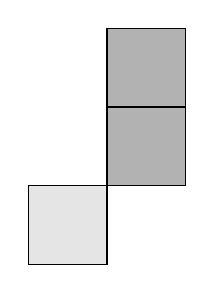
\begin{tikzpicture}
    \draw[fill=black!10] (0,0) grid (1,1) rectangle (0,0);
    \draw[fill=black!30] (1,1) grid (2,3) rectangle (1,1);
  \end{tikzpicture}
\end{center}

\item Nets \textbf{cannot connect along an edge} to other nets,
      as in this example.


\begin{center}
  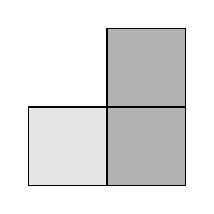
\begin{tikzpicture}
    \draw[fill=black!10] (0,0) grid (1,1) rectangle (0,0);
    \draw[fill=black!30] (1,0) grid (2,2) rectangle (1,0);
  \end{tikzpicture}
\end{center}
\end{enumerate}

You've been provided with an \textbf{Expedition Zone Map}. Each square
on this map that contains a number represents a \mappMobimon{} with
that much strength.
\textbf{Maximize the sum of the numbers covered by your Nets},
and you'll prove you have what it takes to become a \mappMobimon{} Champion!

\phWorksheet{Expedition Zone Map}

\begin{center}
  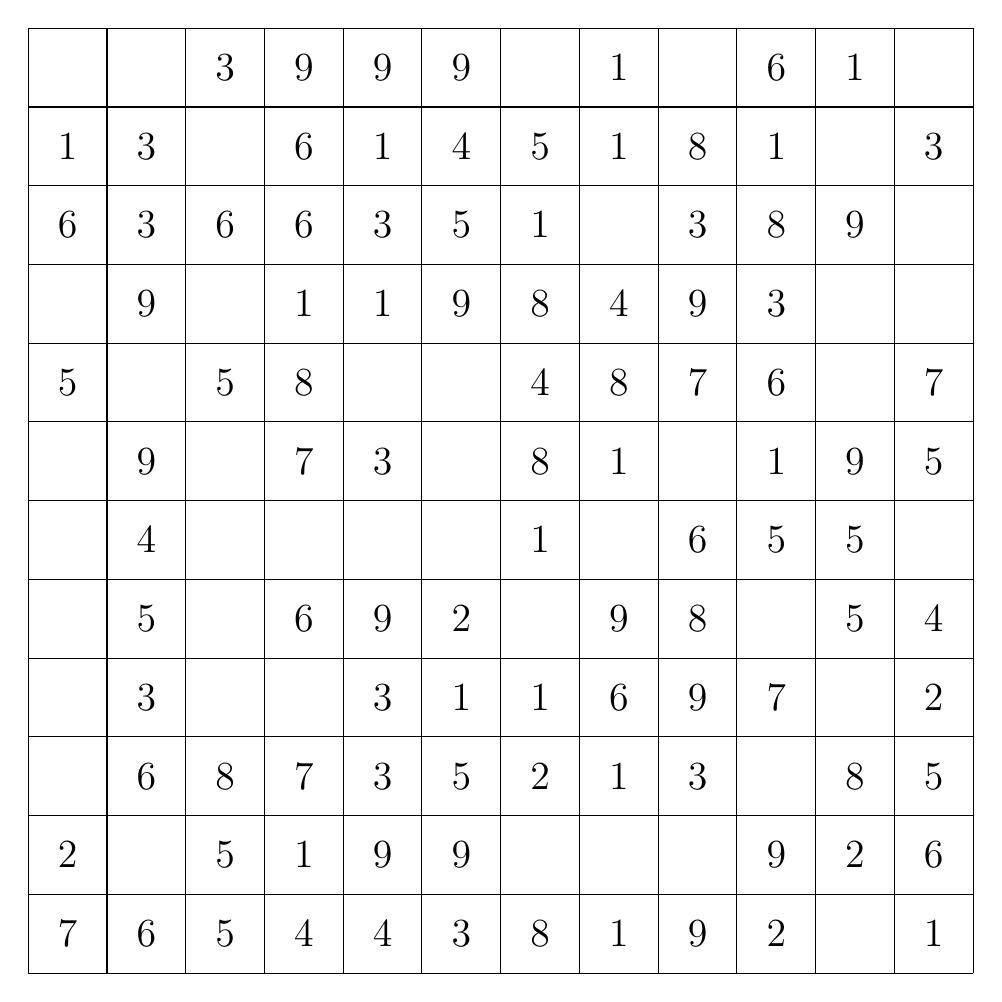
\begin{tikzpicture}
    \draw[step=10mm] (0,0) grid (12,12);

    % nodes - randomly generated by gridgenerator.py
    \tikzstyle{every node}=[font=\Large];
    % run the command:
    % > python gridgenerator.py
    % to generate a new set and copy/paste from gridgen.out (which is a text file
    % despite the unusual extension
    %there are exactly 500 points worth of mobimon
    \node at (5mm, 5mm){7};
    \node at (5mm, 15mm){2};
    \node at (5mm, 75mm){5};
    \node at (5mm, 95mm){6};
    \node at (5mm, 105mm){1};
    \node at (15mm, 5mm){6};
    \node at (15mm, 25mm){6};
    \node at (15mm, 35mm){3};
    \node at (15mm, 45mm){5};
    \node at (15mm, 55mm){4};
    \node at (15mm, 65mm){9};
    \node at (15mm, 85mm){9};
    \node at (15mm, 95mm){3};
    \node at (15mm, 105mm){3};
    \node at (25mm, 5mm){5};
    \node at (25mm, 15mm){5};
    \node at (25mm, 25mm){8};
    \node at (25mm, 75mm){5};
    \node at (25mm, 95mm){6};
    \node at (25mm, 115mm){3};
    \node at (35mm, 5mm){4};
    \node at (35mm, 15mm){1};
    \node at (35mm, 25mm){7};
    \node at (35mm, 45mm){6};
    \node at (35mm, 65mm){7};
    \node at (35mm, 75mm){8};
    \node at (35mm, 85mm){1};
    \node at (35mm, 95mm){6};
    \node at (35mm, 105mm){6};
    \node at (35mm, 115mm){9};
    \node at (45mm, 5mm){4};
    \node at (45mm, 15mm){9};
    \node at (45mm, 25mm){3};
    \node at (45mm, 35mm){3};
    \node at (45mm, 45mm){9};
    \node at (45mm, 65mm){3};
    \node at (45mm, 85mm){1};
    \node at (45mm, 95mm){3};
    \node at (45mm, 105mm){1};
    \node at (45mm, 115mm){9};
    \node at (55mm, 5mm){3};
    \node at (55mm, 15mm){9};
    \node at (55mm, 25mm){5};
    \node at (55mm, 35mm){1};
    \node at (55mm, 45mm){2};
    \node at (55mm, 85mm){9};
    \node at (55mm, 95mm){5};
    \node at (55mm, 105mm){4};
    \node at (55mm, 115mm){9};
    \node at (65mm, 5mm){8};
    \node at (65mm, 25mm){2};
    \node at (65mm, 35mm){1};
    \node at (65mm, 55mm){1};
    \node at (65mm, 65mm){8};
    \node at (65mm, 75mm){4};
    \node at (65mm, 85mm){8};
    \node at (65mm, 95mm){1};
    \node at (65mm, 105mm){5};
    \node at (75mm, 5mm){1};
    \node at (75mm, 25mm){1};
    \node at (75mm, 35mm){6};
    \node at (75mm, 45mm){9};
    \node at (75mm, 65mm){1};
    \node at (75mm, 75mm){8};
    \node at (75mm, 85mm){4};
    \node at (75mm, 105mm){1};
    \node at (75mm, 115mm){1};
    \node at (85mm, 5mm){9};
    \node at (85mm, 25mm){3};
    \node at (85mm, 35mm){9};
    \node at (85mm, 45mm){8};
    \node at (85mm, 55mm){6};
    \node at (85mm, 75mm){7};
    \node at (85mm, 85mm){9};
    \node at (85mm, 95mm){3};
    \node at (85mm, 105mm){8};
    \node at (95mm, 5mm){2};
    \node at (95mm, 15mm){9};
    \node at (95mm, 35mm){7};
    \node at (95mm, 55mm){5};
    \node at (95mm, 65mm){1};
    \node at (95mm, 75mm){6};
    \node at (95mm, 85mm){3};
    \node at (95mm, 95mm){8};
    \node at (95mm, 105mm){1};
    \node at (95mm, 115mm){6};
    \node at (105mm, 15mm){2};
    \node at (105mm, 25mm){8};
    \node at (105mm, 45mm){5};
    \node at (105mm, 55mm){5};
    \node at (105mm, 65mm){9};
    \node at (105mm, 95mm){9};
    \node at (105mm, 115mm){1};
    \node at (115mm, 5mm){1};
    \node at (115mm, 15mm){6};
    \node at (115mm, 25mm){5};
    \node at (115mm, 35mm){2};
    \node at (115mm, 45mm){4};
    \node at (115mm, 65mm){5};
    \node at (115mm, 75mm){7};
    \node at (115mm, 105mm){3};
  \end{tikzpicture}

  \vfill

  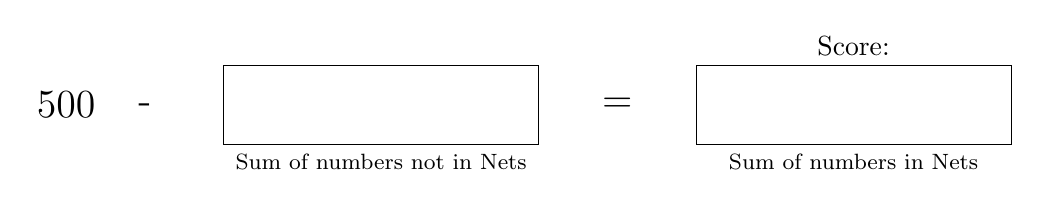
\begin{tikzpicture}
    \node at (0,0) {\Large 500};
    \node at (1,0) {\Large -};
    \draw (2,-0.5) rectangle (6,0.5);
    \node[anchor=north] at (4,-0.5) {\footnotesize Sum of numbers not in Nets};
    \node at (7,0) {\Large =};
    \draw (8,-0.5) rectangle (12,0.5);
    \node[anchor=north] at (10,-0.5) {\footnotesize Sum of numbers in Nets};
    \node[anchor=south] at (10,0.5) {Score:};
  \end{tikzpicture}

  \vfill
\end{center}

\phWorksheet{Mob\'i Nets}

Cut out these figures and tape them to the \textbf{Expedition Zone Map},
following the rules outlined in the \textbf{Bonus Puzzle}.

\begin{center}
  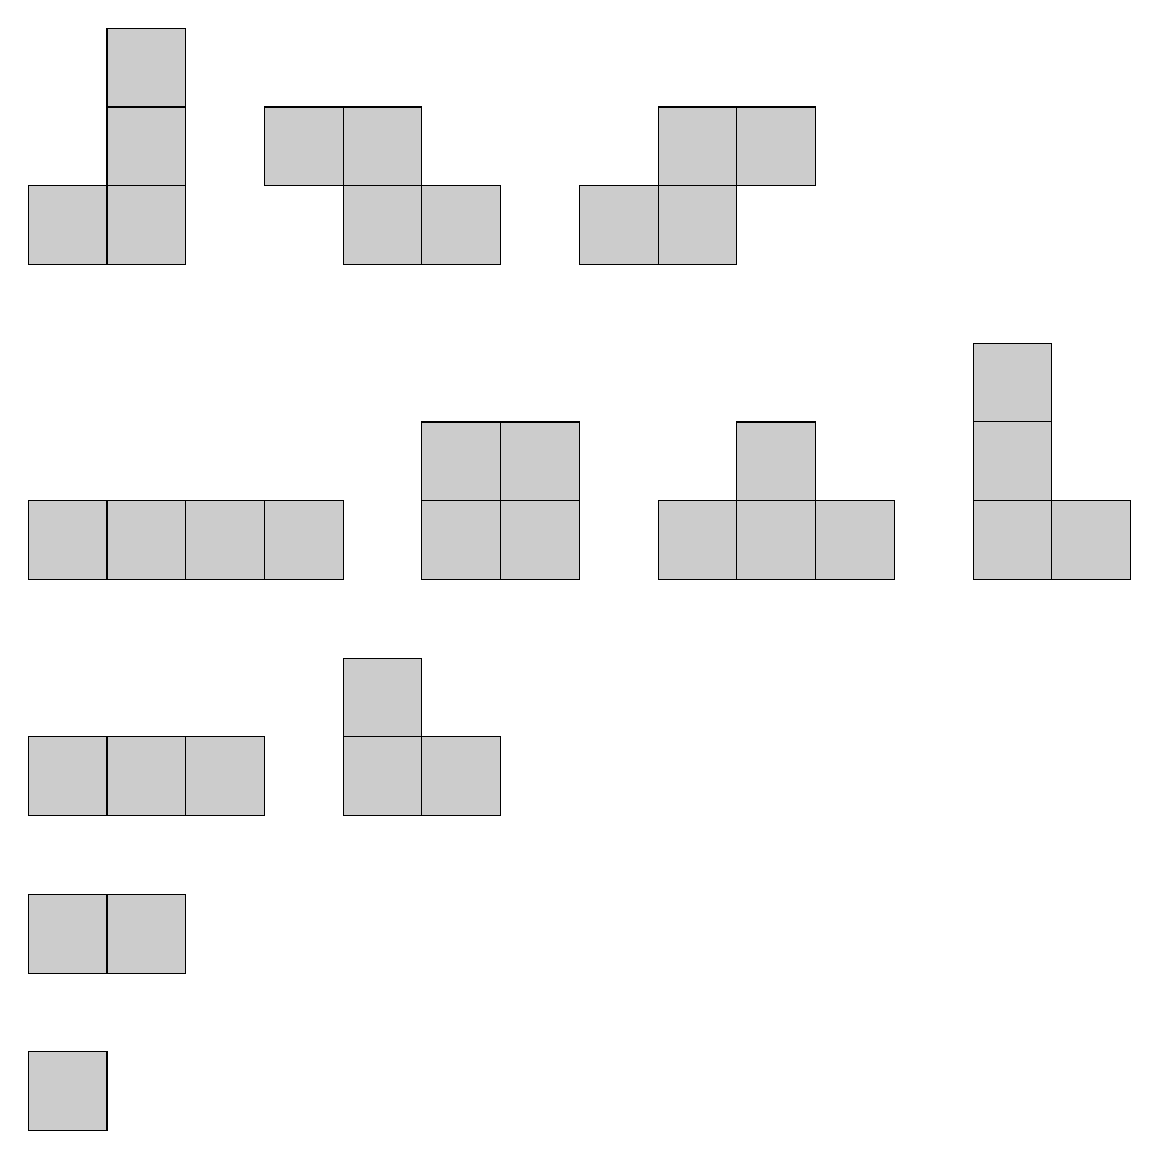
\begin{tikzpicture}
    % trailing rectangle is needed for filling with color
    % monomino
    \draw[step=10mm, fill=black!20] (0, -2) grid (1,-1) rectangle (0,-2);

    % domino
    \draw[step=10mm, fill=black!20] (0,0) grid (2,1) rectangle (0,0);

    % trominoes
    %% I
    \draw[step=10mm, fill=black!20] (0,2) grid (3,3) rectangle (0,2);
    %% L
    \draw[step=10mm, fill=black!20] (4,2) grid (6,3) rectangle (4,2);
    \draw[step=10mm, fill=black!20] (4,3) grid (5,4) rectangle (4,3);

    % tetraminoes
    %% I
    \draw[step=10mm, fill=black!20] (0,5) grid (4,6) rectangle (0,5);
    %% O
    \draw[step=10mm, fill=black!20] (5,5) grid (7,7) rectangle (5,5);
    %% T
    \draw[step=10mm, fill=black!20] (8,5) grid (11,6) rectangle (8,5);
    \draw[step=10mm, fill=black!20] (9,6) grid (10,7) rectangle (9,6);
    %% L
    \draw[step=10mm, fill=black!20] (12,5) grid (13,8) rectangle (12,5);
    \draw[step=10mm, fill=black!20] (13,5) grid (14,6) rectangle (13,5);
    %% J
    \draw[step=10mm, fill=black!20] (0,9) grid (2,10) rectangle (0,9);
    \draw[step=10mm, fill=black!20] (1,10) grid (2,12) rectangle (1,10);
    %% Z
    \draw[step=10mm, fill=black!20] (3,10) grid (5,11) rectangle (3,10);
    \draw[step=10mm, fill=black!20] (4,9) grid (6,10) rectangle (4,9);
    %% S
    \draw[step=10mm, fill=black!20] (7,9) grid (9,10) rectangle (7,9);
    \draw[step=10mm, fill=black!20] (8,10) grid (10,11) rectangle (8,10);
  \end{tikzpicture}
\end{center}

% Include below for aucTeX integration
%%% Local Variables:
%%% mode: latex
%%% TeX-master: "../mapp-challenge-18-game-book"
%%% End:



\phPart{Cryptic Puzzles}

\phChapterWorksheet{Civic Duty}{Mobimon tamers need your help!}

The Mobimon in \textbf{Wenge} are running wild! All of the city utilities that
are powered by Mobimon are offline. The citizens of Wenge don't have
electricity, clean water, or even cell phone signal! \textbf{Eight utilities} have
been disrupted in total.
\begin{enumerate}
\item Electricity, powered by the lightning Mobimon \textbf{Electrumble},
\item water, powered by the moisture Mobimon \textbf{Floobles},
\item traffic lights, controlled by the temporal Mobimon \textbf{Tiktok},
\item garbage, incinerated by the flame Mobimon \textbf{Burnie},
\item cell phone access, routed by the data Mobimon \textbf{Ayepey},
\item sewage, treated by the filter Mobimon \textbf{Stankgunk},
\item street lights, controlled by the photosensitive Mobimon \textbf{Forluxi},
\item and ambulance sirens, controlled by the noisy Mobimon \textbf{Sonitus}.
\end{enumerate}


Luckily Wenge has 86 Mobimon tamers on staff and they will need \textbf{all of
  them} to restore service. They've picked up a few tricks for \textbf{how many
  tamers} should work with each different utility Mobimon.

\begin{itemize}
\item Forluxi needs the fewest tamers.
\item Tiktok needs the most tamers.
\item Ayepey and Sonitus need the same number of tamers. No other two Mobimon
  need the same number of tamers.
\item The number of tamers needed by Burnie and Forluxi differ by one.
\item Burnie and Ayepey need 9 trainers between the two of them.
\end{itemize}

The four strongest of the utility Mobimon need some \textbf{extra tricks}!

\begin{itemize}
\item Each of Electrumble, Floobles, Tiktok, and Stankgunk need a two-digit
  number of tamers.
\item Eletrumble is particularly picky, and needs a perfect square number of
  tamers.
\item Electrumble, Floobles, and Stankgunk each need an even number of tamers.
\item The number of tamers needed by Electrumble and the number of tamers needed
  by Floobles has something in \textbf{common}.
\item The number of tamers needed by Floobles and the number of tamers needed by
  Tiktok also has something in \textbf{common}.
\item The number of tamers needed by Tiktok and the number of tamers needed by
  Stankgunk also has something in \textbf{common}!
\item But the number of tamers needed by Tiktok and the number of tamers needed
  by Electrumble doesn't have much in common.
\end{itemize}

Every Mobimon adventure is about becoming the very best, and helping out the
city of Wenge should tell you something about \textbf{what kind of trait a
  Mobimon champion should have}. Also, the mayor promised to give you his
\textbf{strongest Mobimon} as a reward! Sweet!


% Include below for aucTeX integration
%%% Local Variables:
%%% mode: latex
%%% TeX-master: "../mapp-challenge-18-game-book"
%%% End:

%!TEX root =../mapp-challenge-18-game-book.tex
% ^ leave for LaTeXTools build functionality

\phChapterWorksheet{Cross Products}{Cryptic Puzzle 2}

(angry Dojo Master has a mixed up word search like Puzzle A in VBPuzzlehunt)


% Include below for aucTeX integration
%%% Local Variables:
%%% mode: latex
%%% TeX-master: "../mapp-challenge-18-game-book"
%%% End:

%!TEX root =../mapp-challenge-18-game-book.tex
% ^ leave for LaTeXTools build functionality

\phChapterWorksheet{Blind Luck}{Strange Tilework}

\begin{center}
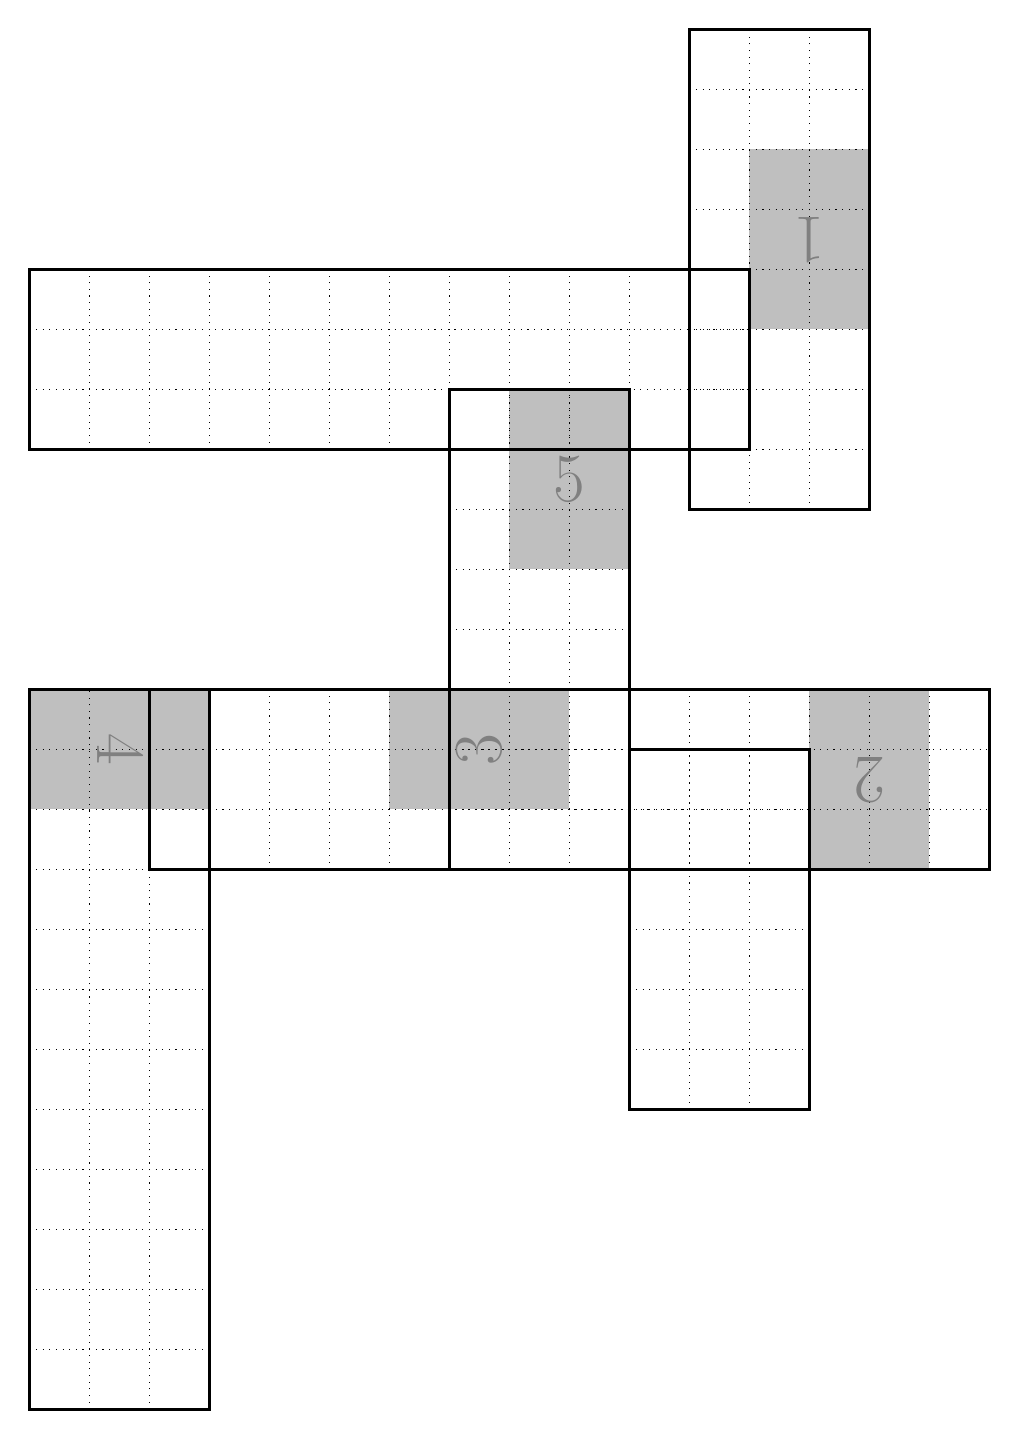
\begin{tikzpicture}[x=0.3in,y=0.3in]
  \fill[color=lightgray] (8,14) rectangle (10,17);
  \fill[color=lightgray] (0,10) rectangle (3,12);
  \fill[color=lightgray] (6,10) rectangle (9,12);
  \fill[color=lightgray] (13,9) rectangle (15,12);
  \fill[color=lightgray] (12,18) rectangle (14,21);

  \blindCrissCrossEntry{(0,0)}{(3,12)};
  \blindCrissCrossEntry{(2,9)}{(16,12)};
  \blindCrissCrossEntry{(10,5)}{(13,11)};
  \blindCrissCrossEntry{(7,9)}{(10,17)};
  \blindCrissCrossEntry{(0,16)}{(12,19)};
  \blindCrissCrossEntry{(11,15)}{(14,23)};

  \node at (9,15.5) {\Huge\rotatebox{0}{\textcolor{gray}{5}}};
  \node at (1.5,11) {\Huge\rotatebox{-90}{\textcolor{gray}{4}}};
  \node at (7.5,11) {\Huge\rotatebox{90}{\textcolor{gray}{3}}};
  \node at (14,10.5) {\Huge\rotatebox{180}{\textcolor{gray}{2}}};
  \node at (13,19.5) {\Huge\rotatebox{180}{\textcolor{gray}{1}}};
\end{tikzpicture}
\end{center}


% Include below for aucTeX integration
%%% Local Variables:
%%% mode: latex
%%% TeX-master: "../mapp-challenge-18-game-book"
%%% End:

%!TEX root =../mapp-challenge-18-game-book.tex
% ^ leave for LaTeXTools build functionality

\phChapterWorksheet{Pin it Down}{Cryptic Puzzle 4}

After figuring out the mysteries of the Doppl \mappMobimon{}, you realize
that they are \textbf{trying to tell you something}. Could it be the location of
a \mappMobimon{} Dojo?! (Of course it is.)

Sure enough, at the end of Road \(\frac{19!}{18!}\), you find the Dojo.
The \textbf{Dojo Master} doesn't hestiate; as soon as you enter her lair,
she sends out two of the most ferocious \mappMobimon{} you've faced yet!

\begin{center}
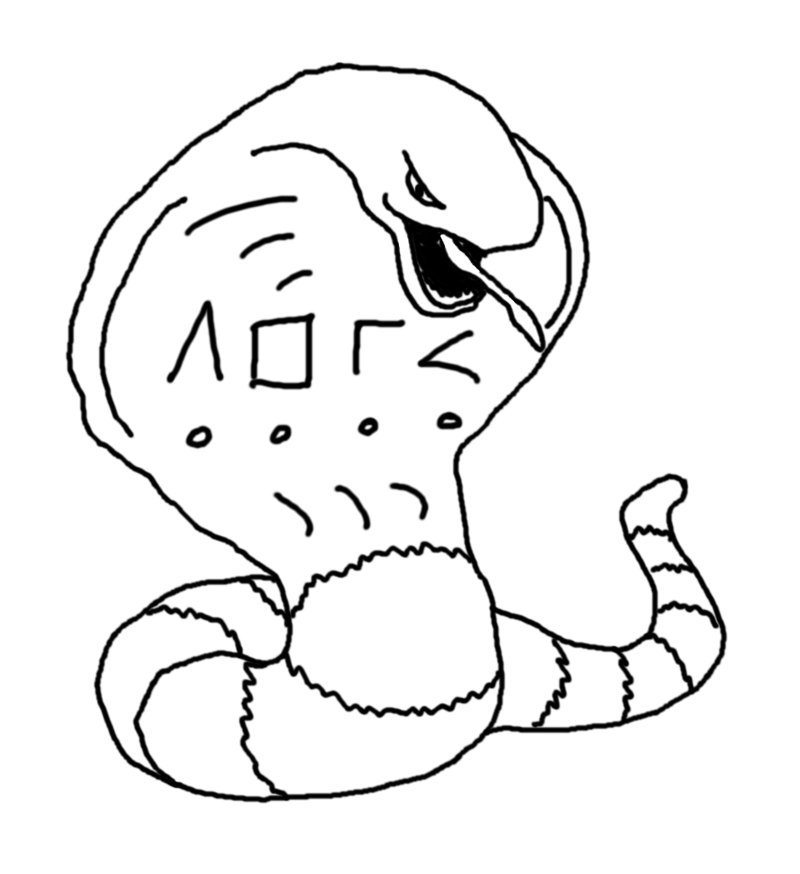
\includegraphics[width=0.4\linewidth]{assets/not-arbok-1.png}
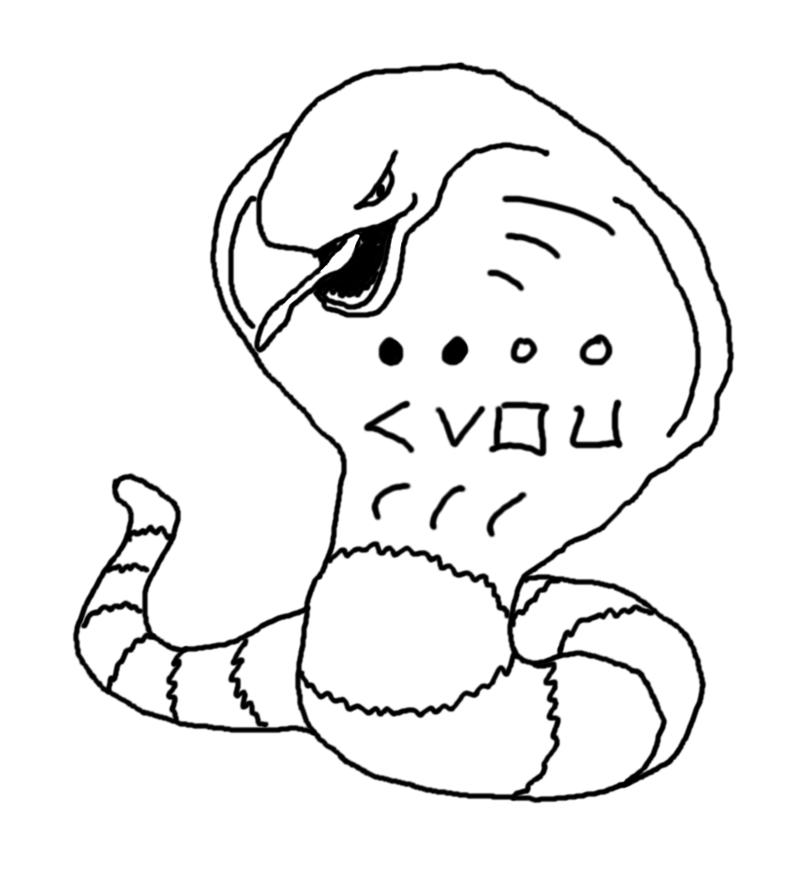
\includegraphics[width=0.4\linewidth]{assets/not-arbok-2.png}
\end{center}

She laughs arrogantly at your hesitation.
``There's something you must first become before you can defeat
my sweet Nohtyp and Doppl!'' Mesmerized, you look for a clue in the arena,
anything that can reveal what you want, no, need to be...


% Include below for aucTeX integration
%%% Local Variables:
%%% mode: latex
%%% TeX-master: "../mapp-challenge-18-game-book"
%%% End:


\phPart{Metapuzzle}
%!TEX root =../mapp-challenge-18-game-book.tex
% ^ leave for LaTeXTools build functionality

\phChapterWorksheet{Route to Victory}{Metapuzzle}

You've finally reached the end of your journey, having been honored
by the four \textbf{Dojo Masters} with the opportunity to compete with them
and three other trainers in the \textbf{\mappMobimon{} Tournament}! You've
each been ranked according to your previous battle experience; unfortunately,
that means you'll have to work your way up from the bottom!

\begin{center}
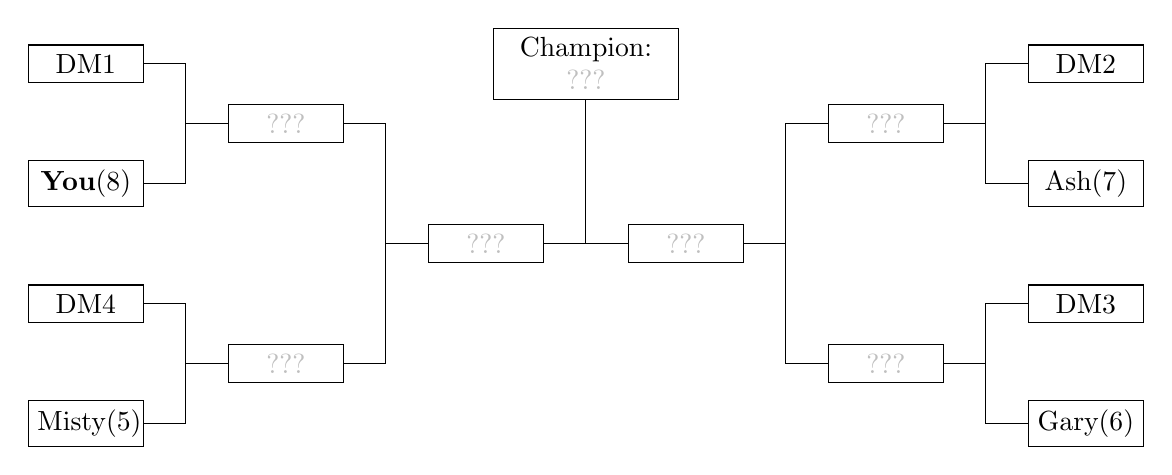
\begin{tikzpicture}[x=0.5in,y=0.3in,every node/.style={rectangle,fill=white,draw,align=center,text width=3.5em}]
  \draw (0,0) -- (1,0) -- (1,1) -- (3,1) -- (3,3) -- (7,3) --
        (7,1) -- (9,1) -- (9,0) -- (10,0);
  \draw (0,2) -- (1,2) -- (1,1);
  \draw (10,2) -- (9,2) -- (9,1);
  \draw (0,6) -- (1,6) -- (1,5) -- (3,5) -- (3,3);
  \draw (10,6) -- (9,6) -- (9,5) -- (7,5) -- (7,3);
  \draw (0,4) -- (1,4) -- (1,5);
  \draw (10,4) -- (9,4) -- (9,5);
  \draw (5,6) -- (5,3);
  \node at (0,6) {DM1};
  \node at (0,4) {\textbf{You}(8)};
  \node at (0,2) {DM4};
  \node at (0,0) {Misty(5)};
  \node at (2,1) {\textcolor{black!25}{???}};
  \node at (2,5) {\textcolor{black!25}{???}};
  \node at (4,3) {\textcolor{black!25}{???}};
  \node[text width=6em] at (5,6) {Champion: \textcolor{black!25}{???}};
  \node at (6,3) {\textcolor{black!25}{???}};
  \node at (8,1) {\textcolor{black!25}{???}};
  \node at (8,5) {\textcolor{black!25}{???}};
  \node at (10,6) {DM2};
  \node at (10,4) {Ash(7)};
  \node at (10,2) {DM3};
  \node at (10,0) {Gary(6)};
\end{tikzpicture}
\end{center}

\begin{multicols}{2}\small
\begin{itemize}
  \item Dojo Master 1 (Rank 1) will use \underline{\hspace{6em}}.
  \item Dojo Master 2 (Rank 2) will use \underline{\hspace{6em}}.
  \item Dojo Master 3 (Rank 3) will use \underline{\hspace{6em}}.
  \item Dojo Master 4 (Rank 4) will use \underline{\hspace{6em}}.
  \item Misty (Rank 5) will use Squidiny.
  \item Gary (Rank 6) will use Glowmage.
  \item Ash (Rank 7) will use Steinape.
  \item You (Rank 8) will use \underline{\hspace{6em}}.
\end{itemize}
\begin{itemize}
  \item 1st place \mappMobimon{}: \underline{\hspace{10em}}
  \item 2nd place \mappMobimon{}: \underline{\hspace{10em}}
  \item 3rd place \mappMobimon{}: \underline{\hspace{10em}}
  \item 4th place \mappMobimon{}: \underline{\hspace{10em}}
  \item 5th place \mappMobimon{}: \underline{\hspace{10em}}
  \item 6th place \mappMobimon{}: \underline{\hspace{10em}}
  \item 7th place \mappMobimon{}: \underline{\hspace{10em}}
  \item 8th place \mappMobimon{}: \underline{\hspace{10em}}
\end{itemize}
\end{multicols}

Your task is no simple one, so be sure to read over the
\textbf{\mappMobimon{} Battling Overview} to learn the ins and outs
of the tournament.

\begin{itemize}
  \item You should be able to \textbf{figure out which \mappMobimon{}} each of
        the Dojo Masters will use in this tournament
        based upon your previous experiences with them and the provided
        \textbf{\mappMobimon{} List}.
  \item You'll also need to \textbf{choose a \mappMobimon{} for yourself}.
        Luckily, there's exactly one \mappMobimon{} on the provided list that
        can beat every trainer you'll face in the tournament!
  \item Finally, if you \textbf{rank the participating \mappMobimon{}} according
        to the tournament results, you might be able to identify an alternate
        title for the \mappMobimon{} Champion, solving today's final
        puzzle!
\end{itemize}


\phWorksheet{\mappMobimon{} Battling Overview}

The \(PWR\) of a \mappMobimon{} move is based on the
\mappMobimon{}'s \(LV\), but modified by a couple rules.

Each \mappMobimon{} has one or two of these types: Ordinary, Flame, Aqua, Plant,
Magic, Undead, and Lightning. In addition, each \mappMobimon{} move has one
of those types as well. If the type of the move matches one of its user's
types, then the \(PWR\) of that move is multiplied by \(1.5\). Otherwise
the \mappMobimon{} type does not affect the \(PWR\) of the move at all.

Secondly, the type(s) of the opponent \mappMobimon{} also affect the move's
\(PWR\), according to the following chart.
For each of the opponent's types, consider the cell found in the
intersection of that column and the row given by the move type. If the cell
isn't empty, multiply the move's \(PWR\) by that number.

\begin{center}
\begin{tabular}{c||c|c|c|c|c|c|c|}
     &  O  &  F  &  A  &  P  &  M  &  U  &  L  \\\hline\hline
  O  &     &     &     &     & 1/2 &  0  & 1/2 \\\hline
  F  &     & 1/2 & 1/2 &  2  &     &  2  &     \\\hline
  A  &     &  2  & 1/2 & 1/2 &  2  &     &     \\\hline
  P  &     & 1/2 &  2  & 1/2 &     &     &  2  \\\hline
  M  & 1/2 &  2  &     &     &     &     &  2  \\\hline
  U  &  0  &     &     &  2  &  2  &     &     \\\hline
  L  & 1/2 &     &  2  &     &     &  2  &     \\\hline
\end{tabular}
\end{center}

For example, a Flame-type move used against a Plant/Magic-type
\mappMobimon{} is modified by a factor of \(2\), but it
would be modified by \(\frac{1}{4}\) instead if used against a Flame/Aqua-type
\mappMobimon{}. (If the user has the Flame type, then the total modifers would
be \(3\) and \(\frac{3}{8}\), respectively.)

Each \mappMobimon{} knows two different moves, so it's up to the
trainer to decide which move would have greater \(PWR\) against their
opponent. The \mappMobimon{} that uses the move with greater \(PWR\) than
their opponent wins the battle and moves on in the tournament, and the
loser is knocked out.

During a tournament, each trainer must use the same \mappMobimon{} for all
battles, and each \mappMobimon{} cannot be used by more than one trainer.
At the conclusion of the tournament, the trainers and their
\mappMobimon{} are ranked according
to how many battles were won: 1st place for 3 wins, 2nd place for 2 wins,
3rd-4th place for 1 win, and 5th-8th place for no wins. The rankings each
trainer entered the tournament with are used to sort 3rd-4th and 5th-8th
places.

\phWorksheet{\mappMobimon{} List}

\begin{center}
\begin{tabular}{|c|c|c|c|c|p{2in}|}\hline
  Name & Type(s) & \(LV\) & 1st Move & 2nd Move & Mob\'idex Description \\\hline\hline
  %%%%%%%%%%%%%%%%%%%%%%%%%%%%%%%%%%%%%%%%%%%%%%%%%%%%%%%%%%%%%%%%%%%%%%
  Ariafire & Flame & 50 & Flame & Lightning &
    Works well with other firey \mappMobimon{}. \\\hline
  Burnezam & Flame/Magic & 49 & Flame & Magic &
    Known for its caution and level-headedness. \\\hline
  Dawnoduh & Ordinary/Undead & 56 & Ordinary & Flame &
    Your run-of-the-mill zombie. \\\hline
  Emaphant & Ordinary & 52 & Ordinary & Magic &
    Tramples over the competition. \\\hline
  Finfanta & Magic & 54 & Magic & Flame &
    Moody, it creates clouds of strife. \\\hline
  Glowmage & Magic/Lightning & 55 & Magic & Undead &
    A shining example of magical prowess. \\\hline
  Planktin & Aqua/Plant & 51 & Plant & Ordinary &
    Well, it grows on you at least. \\\hline
  Scorchar & Flame/Lightning & 58 & Flame & Undead &
    It can run a marathon in under 38 minutes. \\\hline
  Steinape & Undead/Lightning & 47 & Lightning & Ordinary &
    It's alive with passion for battling. \\\hline
  Squidiny & Aqua & 57 & Aqua & Ordinary &
    A lot of fun to go surfing with. \\\hline
  Thundora & Lightning & 53 & Lightning & Plant &
    This extreme \mappMobimon{} pushes it to the limit. \\\hline
  Zomtreed & Plant/Undead & 43 & Undead & Magic &
    Incredibly profecient, like no one ever was. \\\hline
\end{tabular}
\end{center}


% Include below for aucTeX integration
%%% Local Variables:
%%% mode: latex
%%% TeX-master: "../mapp-challenge-18-game-book"
%%% End:


\phPart{Appendex}
\phChapter{Solutions}
%!TEX root =../mapp-challenge-18-game-book.tex
% ^ leave for LaTeXTools build functionality

\phSection{Main Puzzle 1 - Go Get 'Em}

The correct stones are laid as follows.

\begin{multicols}{3}
\begin{itemize}
  \item Black on JT - \texttt{T}
  \item White on HQ - \texttt{H}
  \item White on EZ - \texttt{E}
  \item White on FP - \texttt{F}
  \item Black on BO - \texttt{O}
  \item Black on ER - \texttt{R}
  \item White on EO - \texttt{E}
  \item Black on GS - \texttt{S}
  \item Black on ET - \texttt{T}
\end{itemize}
\end{multicols}

The solution is \texttt{THEFOREST}.

\phSection{Main Puzzle 2 - When Push Comes to Shove}



\begin{multicols}{2}
  \begin{itemize}
    \item \texttt{M=13=2+11}
      The number of ways you can stack either \(2\) or \(6\) boxes.
    \item \texttt{O=15}
      The number of ways you can stack \(12\) boxes, if every row must
      contain an odd number.
    \item \texttt{U=21=22-1}
      The number of ways you can stack \(8\) boxes, if every row must contain
      less than eight.
    \item \texttt{S=19=1+1+2+3+5+7}
      The number of ways you can stack up to \(5\) boxes. (An empty room
      counts as one way...)
    \item \texttt{E=5}
      The number of ways you can stack \(4\) boxes.
  \end{itemize}
\columnbreak
  \begin{itemize}
    \item \texttt{T=20=22-2}
      The number of ways you can stack \(8\) boxes, if every row must contain
      less than seven.
    \item \texttt{R=18}
      The number of ways you can stack \(13\) boxes, if every row must have
      less boxes than the row below it.
    \item \texttt{A=1}
      The number of ways you can stack \(42\) boxes, if you can only use one
      row.
    \item \texttt{P=16=1+15}
      The number of ways you can stack \(1\) or \(12\) boxes, if every row must
      have a unique number of boxes.
  \end{itemize}
\end{multicols}

The solution is \texttt{MOUSETRAP}.

\phSection{Main Puzzle 3 - The Name Rater}

Since vowels are always doubled or subtracted by \(3\) when creating
excellent nicknames, and the basic excellent nicknames
have exactly one vowel, it is impossible for an excellent nickname
to have a multiple of \(3\) vowels in a word.
Thus all the words that have \(3\) vowels are not excellent (and the
others can be verified to be excellent).

\begin{multicols}{2}
  \begin{itemize}
    \item \textbf{MANKAY} \texttt{4As->BA->B->BABBAB}
    \item \textit{ULTRAMON} (3 vowels)
    \item \textbf{OMASTARE} \texttt{16As->ABABBABA}
    \item \textit{VOLTEON} (3 vowels)
    \item \textit{GENGASKHAN} (3 vowels)
    \item \textit{EEVOL} (3 vowels)
    \item \textbf{NOHTYP} \texttt{16As->BABBBB}
    \item \textit{BLASTMOIST} (3 vowels)
    \item \textbf{ICHU} \texttt{8As->ABBA}
    \item \textbf{KADABARA} \texttt{4As->BA->BABABABA}
    \item \textit{AERODYCTL} (3 vowels)
    \item \textit{PARACENT} (3 vowels)
    \item \textbf{EARSEA} \texttt{16As->AABBAABB->AABBAA}
    \item \textit{DRAGONAT} (3 vowels)
    \item \textbf{RAGMAR} \texttt{4As->BA->BAB->BABBAB}
  \end{itemize}
\end{multicols}

The solution \texttt{MONIKER} is another word for nickname
(but is not excellent as a nickname, because it has 3 vowels).

\phSection{Main Puzzle 4 - An Unending Enigma}

\begin{align*}
  (\omega+3)\cdot(\omega+5)&=\omega^2\cdot E+\omega\cdot G+S
                            =\omega^2\cdot 1+\omega\cdot 5+3 \\
  \omega+1+\omega+3+\omega+5+\omega+7&=\omega\cdot I+O
                                      =\omega\cdot 4+7 \\
  3\cdot\omega+\omega^2\cdot 5+4\cdot(\omega^2+2)&=
        \omega^2\cdot L+\omega\cdot R+N =
        \omega^2\cdot 6+\omega\cdot 0+8 \\
  2\cdot(2+\omega\cdot3)+(\omega\cdot3+2)\cdot2&=
        \omega\cdot A+M =
        \omega\cdot 9+2
\end{align*}

This yields the solution \texttt{24007042951=MIRRORIMAGE}.

\phSection{Cryptic Puzzle 1 - Civic Duty}

This puzzle is solved by ordering the \mappMobimon{} alphabetically,
then converting the required number of trainers using A=1,B=2, etc.

\begin{multicols}{2}
\begin{itemize}
  \item {Ayepey}: \(P=16\)
  \item {Burnie}: \(R=18\)
  \item {Corporil}: \(U=21\)
  \item {Dankgunk}: \(D=4\)
  \item {Electrumble}: \(E=5\)
  \item {Forluxi}: \(N=14\)
  \item {Glooble}: \(C=3\)
  \item {Hearit}: \(E=5\)
\end{itemize}
\end{multicols}

The solution is \texttt{PRUDENCE}.

\phSection{Cryptic Puzzle 2 - Cross Product}

``Only a trainer that has one of these can possibly become CHIPONAM.''
\texttt{CHIPONAM} is an anagram of \texttt{CHAMPION}, hinting players to
search for anagrams of the seven given words within the grid.

\begin{center}
\resizebox{2in}{!}{
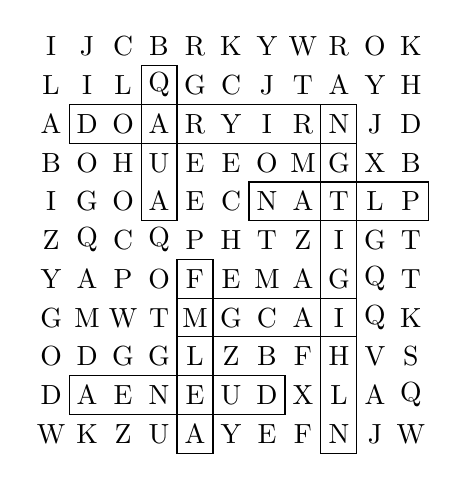
\begin{tikzpicture}[x=1.3em,y=1.4em]
  \node at (0,11) {I};\node at (1,11) {J};\node at (2,11) {C};\node at (3,11) {B};\node at (4,11) {R};\node at (5,11) {K};\node at (6,11) {Y};\node at (7,11) {W};\node at (8,11) {R};\node at (9,11) {O};\node at (10,11) {K};
  \node at (0,10) {L};\node at (1,10) {I};\node at (2,10) {L};\node at (3,10) {Q};\node at (4,10) {G};\node at (5,10) {C};\node at (6,10) {J};\node at (7,10) {T};\node at (8,10) {A};\node at (9,10) {Y};\node at (10,10) {H};
  \node at (0,9) {A};\node at (1,9) {D};\node at (2,9) {O};\node at (3,9) {A};\node at (4,9) {R};\node at (5,9) {Y};\node at (6,9) {I};\node at (7,9) {R};\node at (8,9) {N};\node at (9,9) {J};\node at (10,9) {D};
  \node at (0,8) {B};\node at (1,8) {O};\node at (2,8) {H};\node at (3,8) {U};\node at (4,8) {E};\node at (5,8) {E};\node at (6,8) {O};\node at (7,8) {M};\node at (8,8) {G};\node at (9,8) {X};\node at (10,8) {B};
  \node at (0,7) {I};\node at (1,7) {G};\node at (2,7) {O};\node at (3,7) {A};\node at (4,7) {E};\node at (5,7) {C};\node at (6,7) {N};\node at (7,7) {A};\node at (8,7) {T};\node at (9,7) {L};\node at (10,7) {P};
  \node at (0,6) {Z};\node at (1,6) {Q};\node at (2,6) {C};\node at (3,6) {Q};\node at (4,6) {P};\node at (5,6) {H};\node at (6,6) {T};\node at (7,6) {Z};\node at (8,6) {I};\node at (9,6) {G};\node at (10,6) {T};
  \node at (0,5) {Y};\node at (1,5) {A};\node at (2,5) {P};\node at (3,5) {O};\node at (4,5) {F};\node at (5,5) {E};\node at (6,5) {M};\node at (7,5) {A};\node at (8,5) {G};\node at (9,5) {Q};\node at (10,5) {T};
  \node at (0,4) {G};\node at (1,4) {M};\node at (2,4) {W};\node at (3,4) {T};\node at (4,4) {M};\node at (5,4) {G};\node at (6,4) {C};\node at (7,4) {A};\node at (8,4) {I};\node at (9,4) {Q};\node at (10,4) {K};
  \node at (0,3) {O};\node at (1,3) {D};\node at (2,3) {G};\node at (3,3) {G};\node at (4,3) {L};\node at (5,3) {Z};\node at (6,3) {B};\node at (7,3) {F};\node at (8,3) {H};\node at (9,3) {V};\node at (10,3) {S};
  \node at (0,2) {D};\node at (1,2) {A};\node at (2,2) {E};\node at (3,2) {N};\node at (4,2) {E};\node at (5,2) {U};\node at (6,2) {D};\node at (7,2) {X};\node at (8,2) {L};\node at (9,2) {A};\node at (10,2) {Q};
  \node at (0,1) {W};\node at (1,1) {K};\node at (2,1) {Z};\node at (3,1) {U};\node at (4,1) {A};\node at (5,1) {Y};\node at (6,1) {E};\node at (7,1) {F};\node at (8,1) {N};\node at (9,1) {J};\node at (10,1) {W};

  \draw (0.5,8.5) rectangle (8.5,9.5);
  \draw (2.5,6.5) rectangle (3.5,10.5);
  \draw (7.5,0.5) rectangle (8.5,9.5);
  \draw (5.5,6.5) rectangle (10.5,7.5);
  \draw (3.5,3.5) rectangle (8.5,4.5);
  \draw (3.5,0.5) rectangle (4.5,5.5);
  \draw (0.5,1.5) rectangle (6.5,2.5);
\end{tikzpicture}
}
\end{center}

Each ``cross product'' represents the letter where the two words cross in
the grid, yielding the following.

\begin{center}
Lightning \(\times\) Plant = T\hfill
Undead \(\times\) Flame = E\hfill
Aqua \(\times\) Ordinary = A\hfill
Flame \(\times\) Magic = M
\end{center}

The solution is \texttt{TEAM}.

\phSection{Cryptic Puzzle 3 - Blind Luck}

The blind/sight clues suggest to find a way to criss-cross the given
words in the grid using Braille. There is exactly one way to do this,
involving various orientations for each word.

\begin{center}
\resizebox{3in}{!}{
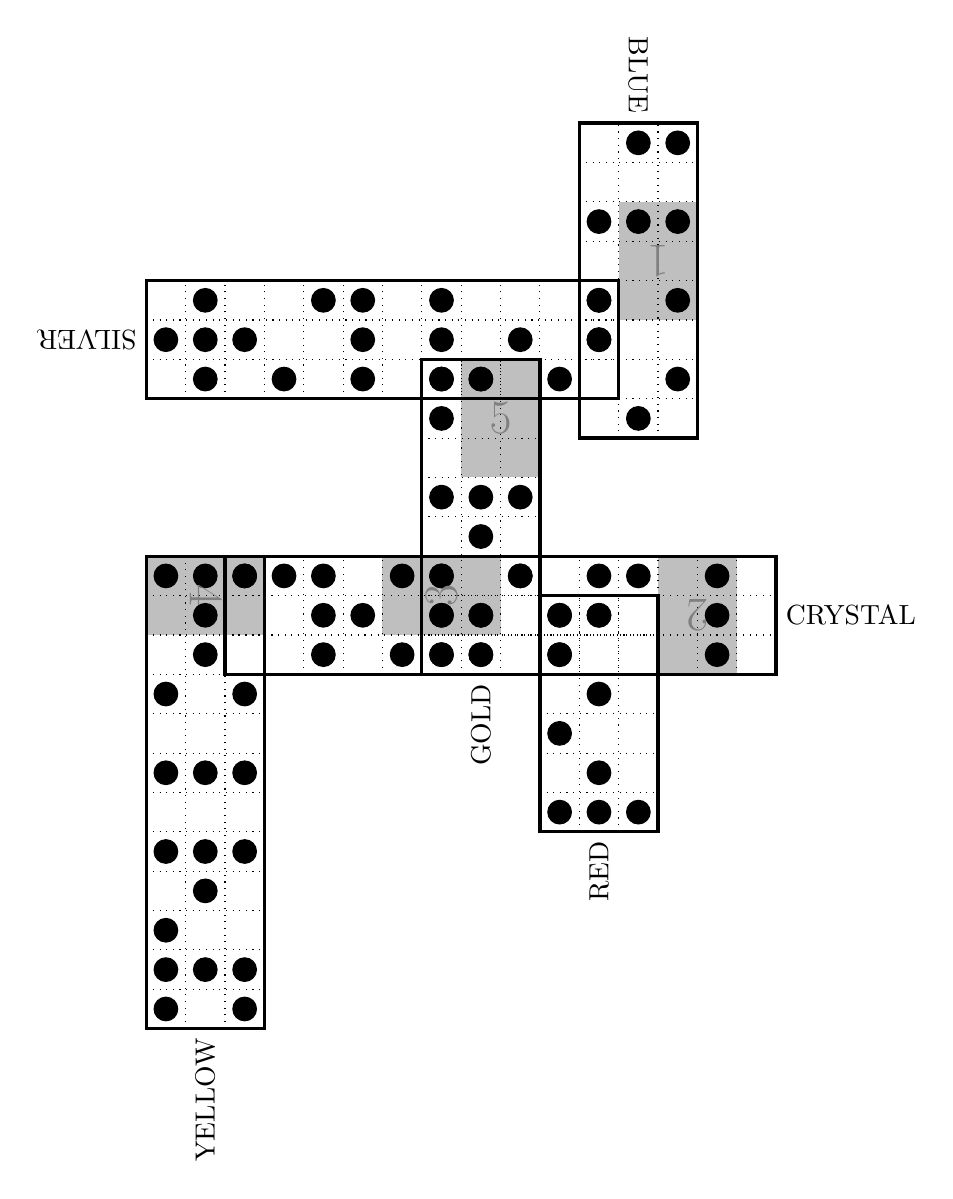
\begin{tikzpicture}[x=0.5cm,y=0.5cm]
  \fill[color=lightgray] (8,14) rectangle (10,17);
  \fill[color=lightgray] (0,10) rectangle (3,12);
  \fill[color=lightgray] (6,10) rectangle (9,12);
  \fill[color=lightgray] (13,9) rectangle (15,12);
  \fill[color=lightgray] (12,18) rectangle (14,21);

  \blindCrissCrossEntry{(0,0)}{(3,12)};
  \blindCrissCrossEntry{(2,9)}{(16,12)};
  \blindCrissCrossEntry{(10,5)}{(13,11)};
  \blindCrissCrossEntry{(7,9)}{(10,17)};
  \blindCrissCrossEntry{(0,16)}{(12,19)};
  \blindCrissCrossEntry{(11,15)}{(14,23)};

  %YELLOW
  \node[anchor=north] at (1.5,0) {\rotatebox{90}{YELLOW}};

  \blindCrissCrossPip{0}{0};
  \blindCrissCrossPip{2}{0};

  \blindCrissCrossPip{0}{1};
  \blindCrissCrossPip{1}{1};
  \blindCrissCrossPip{2}{1};

  \blindCrissCrossPip{0}{2};

  \blindCrissCrossPip{1}{3};

  \blindCrissCrossPip{0}{4};
  \blindCrissCrossPip{1}{4};
  \blindCrissCrossPip{2}{4};

  \blindCrissCrossPip{0}{6};
  \blindCrissCrossPip{1}{6};
  \blindCrissCrossPip{2}{6};

  \blindCrissCrossPip{0}{8};
  \blindCrissCrossPip{2}{8};

  \blindCrissCrossPip{1}{9};

  \blindCrissCrossPip{1}{10};

  \blindCrissCrossPip{0}{11};
  \blindCrissCrossPip{1}{11};
  \blindCrissCrossPip{2}{11};

  %CRYSTAL
  \node[anchor=west] at (16,10.5) {CRYSTAL};
  \blindCrissCrossPip{2}{11};

  \blindCrissCrossPip{3}{11};

  \blindCrissCrossPip{4}{9};
  \blindCrissCrossPip{4}{10};
  \blindCrissCrossPip{4}{11};

  \blindCrissCrossPip{5}{10};

  \blindCrissCrossPip{6}{9};
  \blindCrissCrossPip{6}{11};

  \blindCrissCrossPip{7}{9};
  \blindCrissCrossPip{7}{10};
  \blindCrissCrossPip{7}{11};

  \blindCrissCrossPip{8}{9};
  \blindCrissCrossPip{8}{10};

  \blindCrissCrossPip{9}{11};

  \blindCrissCrossPip{10}{9};
  \blindCrissCrossPip{10}{10};

  \blindCrissCrossPip{11}{10};
  \blindCrissCrossPip{11}{11};

  \blindCrissCrossPip{12}{11};

  \blindCrissCrossPip{14}{9};
  \blindCrissCrossPip{14}{10};
  \blindCrissCrossPip{14}{11};

  %RED
  \node[anchor=north] at (11.5,5) {\rotatebox{90}{RED}};

  \blindCrissCrossPip{10}{5};
  \blindCrissCrossPip{11}{5};
  \blindCrissCrossPip{12}{5};

  \blindCrissCrossPip{11}{6};

  \blindCrissCrossPip{10}{7};

  \blindCrissCrossPip{11}{8};

  \blindCrissCrossPip{10}{9};

  \blindCrissCrossPip{10}{10};
  \blindCrissCrossPip{11}{10};

  %GOLD
  \node[anchor=north] at (8.5,9) {\rotatebox{90}{GOLD}};

  \blindCrissCrossPip{7}{9};
  \blindCrissCrossPip{8}{9};

  \blindCrissCrossPip{7}{10};
  \blindCrissCrossPip{8}{10};

  \blindCrissCrossPip{7}{11};
  \blindCrissCrossPip{9}{11};

  \blindCrissCrossPip{8}{12};

  \blindCrissCrossPip{7}{13};
  \blindCrissCrossPip{8}{13};
  \blindCrissCrossPip{9}{13};

  \blindCrissCrossPip{7}{15};

  \blindCrissCrossPip{7}{16};
  \blindCrissCrossPip{8}{16};

  %SILVER
  \node[anchor=east] at (0,17.5) {\rotatebox{180}{SILVER}};

  \blindCrissCrossPip{11}{18};
  \blindCrissCrossPip{11}{17};

  \blindCrissCrossPip{10}{16};

  \blindCrissCrossPip{9}{17};

  \blindCrissCrossPip{8}{16};

  \blindCrissCrossPip{7}{18};
  \blindCrissCrossPip{7}{17};
  \blindCrissCrossPip{7}{16};

  \blindCrissCrossPip{5}{18};
  \blindCrissCrossPip{5}{17};
  \blindCrissCrossPip{5}{16};

  \blindCrissCrossPip{4}{18};

  \blindCrissCrossPip{3}{16};

  \blindCrissCrossPip{2}{17};

  \blindCrissCrossPip{1}{18};
  \blindCrissCrossPip{1}{17};
  \blindCrissCrossPip{1}{16};

  \blindCrissCrossPip{0}{17};

  %BLUE
  \node[anchor=south] at (12.5,23) {\rotatebox{-90}{BLUE}};

  \blindCrissCrossPip{12}{22};
  \blindCrissCrossPip{13}{22};

  \blindCrissCrossPip{11}{20};
  \blindCrissCrossPip{12}{20};
  \blindCrissCrossPip{13}{20};

  \blindCrissCrossPip{11}{18};
  \blindCrissCrossPip{13}{18};

  \blindCrissCrossPip{11}{17};

  \blindCrissCrossPip{13}{16};

  \blindCrissCrossPip{12}{15};

  \node at (9,15.5) {\LARGE\rotatebox{0}{\textcolor{gray}{5}}};
  \node at (1.5,11) {\LARGE\rotatebox{-90}{\textcolor{gray}{4}}};
  \node at (7.5,11) {\LARGE\rotatebox{90}{\textcolor{gray}{3}}};
  \node at (14,10.5) {\LARGE\rotatebox{180}{\textcolor{gray}{2}}};
  \node at (13,19.5) {\LARGE\rotatebox{180}{\textcolor{gray}{1}}};
\end{tikzpicture}
}
\end{center}

The numbered regions yield \texttt{12345=ULTRA} in Braille.

\phSection{Cryptic Puzzle 4 - Pin It Down}

Overlaying the mirror images of the monsters reveals a message using
the Pig Pen cipher.

\begin{center}
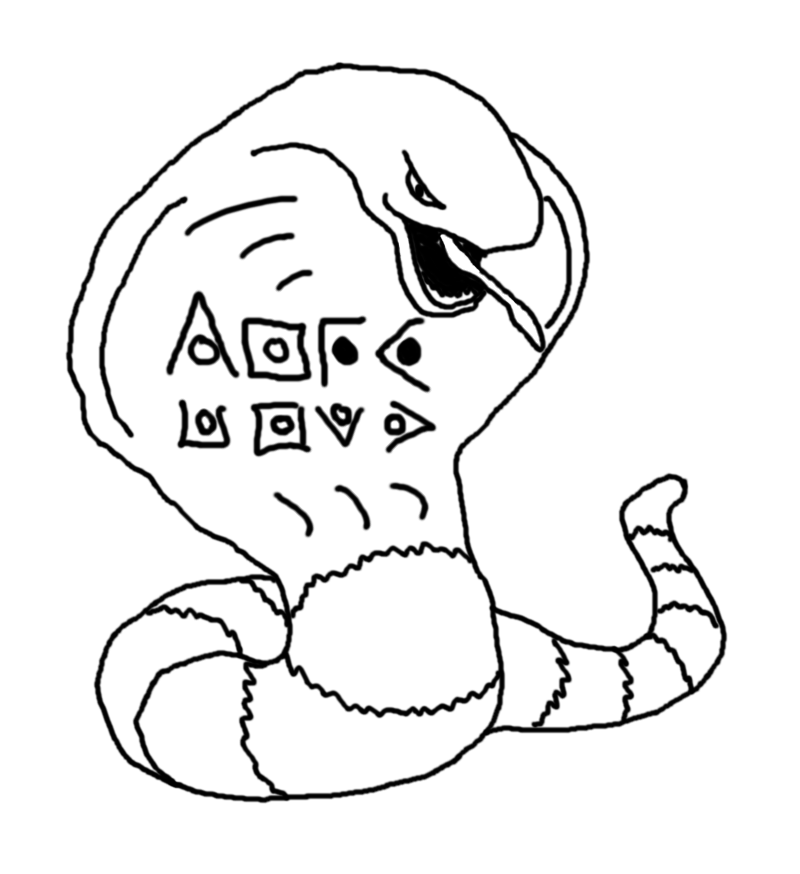
\includegraphics[width=0.4\linewidth]{assets/not-arbok-solution.png}
\end{center}

The solution is \texttt{VERYBEST}.

\phSection{Metapuzzle - The Ultimate Quartet}

%%% Local Variables:
%%% mode: latex
%%% TeX-master: "../mapp-hsc17-game-book"
%%% End:


%!TEX root =../mapp-challenge-18-game-book.tex
% ^ leave for LaTeXTools build functionality

\phChapterWorksheet{Knot True}{Tournament Results}

\begin{center}\Huge
\begin{tikzpicture}[x=0.8in,y=0.8in]
  \draw[line width=2pt] (0,0) rectangle (6,6);
  \draw[step=1] (0,0) grid (6,6);
  \node[anchor=south] at (0.5,6) {\rotatebox{90}{Ash}};
  \node[anchor=south] at (1.5,6) {\rotatebox{90}{Brock}};
  \node[anchor=south] at (2.5,6) {\rotatebox{90}{Cynthia}};
  \node[anchor=south] at (3.5,6) {\rotatebox{90}{Drayden}};
  \node[anchor=south] at (4.5,6) {\rotatebox{90}{Erika}};
  \node[anchor=south] at (5.5,6) {\rotatebox{90}{Flannery}};
  \node[anchor=east] at (0,5.5) {1st};
  \node[anchor=east] at (0,4.5) {2nd};
  \node[anchor=east] at (0,3.5) {3rd};
  \node[anchor=east] at (0,2.5) {4th};
  \node[anchor=east] at (0,1.5) {5th};
  \node[anchor=east] at (0,0.5) {6th};
  \foreach \letters [count=\i] in {
    {O,Y,G,U,S,J},
    {Q,C,M,V,A,X},
    {F,P,U,N,I,E},
    {L,A,S,I,D,T},
    {K,N,B,Z,T,R},
    {H,R,W,E,L,M},
  } {
    \foreach \letter [count=\j] in \letters {
      \node at ($(\j.5,-\i.5)+(-1,7)$) {\letter};
    }
  }
\end{tikzpicture}
\end{center}

\phWorksheet{Ash's Trainer Badge}

  \begin{center}
    
\includegraphics[width=4in]{assets/unknot1.pdf}

    \Huge Trainer ID: 365867

%    Ash and Flannery did not place 6th.
  \end{center}

\phWorksheet{Brock's Trainer Badge}
  \begin{center}

    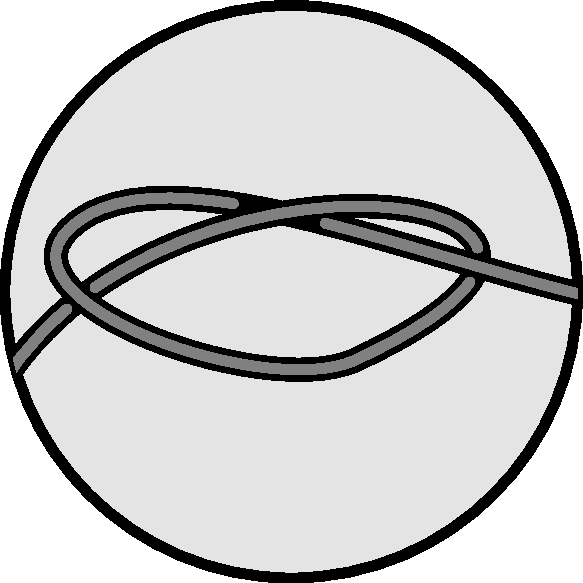
\includegraphics[width=4in]{assets/knot1.pdf}

    \Huge Trainer ID: 198815
%
%    Neither Brock nor Drayden placed 4th.
%
%
  \end{center}

\phWorksheet{Cynthia's Trainer Badge}
  \begin{center}
    
\includegraphics[width=4in]{assets/unknot2.pdf}

    \Huge Trainer ID: 255123 
%
%    Erika placed exactly one rank higher than Ash.
%
  \end{center}

\phWorksheet{Drayden's Trainer Badge}
  \begin{center}
%
    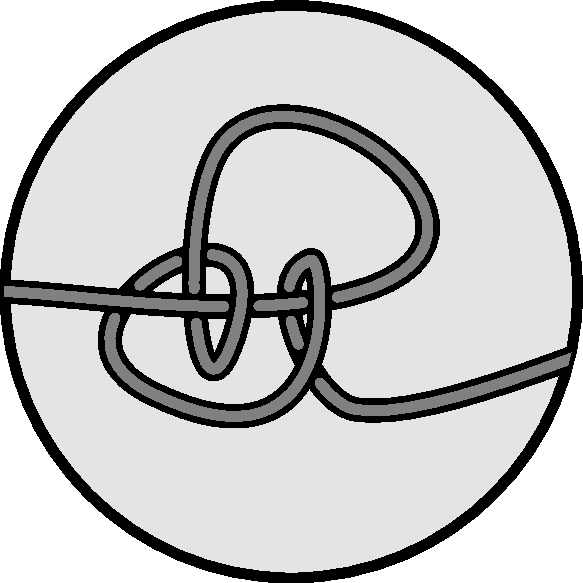
\includegraphics[width=4in]{assets/knot2.pdf}

    \Huge Trainer ID: 443881 
%
%    Drayden placed in the top three.
%
%
  \end{center}

\phWorksheet{Erika's Trainer Badge}
  \begin{center}
    
\includegraphics[width=4in]{assets/knot3.pdf}

    \Huge Trainer ID: 310235 
%
%    Brock placed lower than Flannery.
%
%
  \end{center}

\phWorksheet{Flannery's Trainer Badge}
  \begin{center}
    
\includegraphics[width=4in]{assets/unknot3.pdf}

    \Huge Trainer ID: 663968
%
%    Either Cynthia or Drayden placed 3rd.
  \end{center}



% Include below for aucTeX integration
%%% Local Variables:
%%% mode: latex
%%% TeX-master: "../mapp-challenge-18-game-book"
%%% End:


\phChapter{Credits}
%!TEX root =../mapp-hsc17-game-book.tex
% ^ leave for LaTeXTools build functionality

Thanks for downloading the puzzle booklet for \textbf{\phEventName} by
Mathematical Puzzle Programs.  These puzzle materials are provided as-is for use
in the classroom (or anywhere else!)  to help showcase the fun of mathematical
problem-solving.

When the \phEventName is over, we'd love your feedback on how to improve this
booklet. You can contact us by email at info@mappmath.org. Or better yet, submit
an issue or pull request at our GitHub page at \url{https://github.com/MaPPmath}
directly.

More information on Mathematical Puzzle Programs may be found at our website
\url{http://mappmath.org} and on our Twitter @MaPPmath. Happy mathematical puzzling!

- MaPP Directors and Volunteers

\phSection{Mathematical Puzzle Programs Staff}
  \begin{itemize}
    \item Steven Clontz --- Director
    \item Braxton Carrigan --- Associate Director
    \item PJ Couch --- Associate Director
    \item Zachary Sarver --- \phEventAbbr Game Designer
  \end{itemize}

\phSection{\phEventName Featured Puzzle Designer}
  \begin{itemize}
  \item Eric Harshbarger ---
        Freelance puzzle and game designer, Auburn, AL
  \end{itemize}

\phSection{\phEventName Puzzle Designers}
  \begin{itemize}
  \item PJ Couch ---
        Lamar University, Beaumont, TX
  \item Danielle Dobie ---
        Mathematician and freelance puzzle designer, New Ulm, MN
  \item Christopher Night ---
        Google Inc., Boston, MA
  \item Harold Reiter ---
        University of North Carolina at Charlotte, Charlotte, NC
  \item Zachary Sarver ---
        Auburn University, Auburn, AL
  \end{itemize}

\phSection{Special Thanks}
\begin{itemize}
\item Ronimo Games, for the use of the Awesomenauts brand
      and artwork in Puzzle 4.
\end{itemize}

\phSection{Attribution}

All rights to the original content in this game book are reserved by
Mathematical Puzzle Programs until the conclusion
of all \phEventName competitions.

Following the conclusion of all \phEventName competitions,
Mathematical Puzzle Programs licenses the original content in this game book
under the Creative Commons Attribution 4.0
International License. To view a copy of this license, visit the following URL.

\begin{center}
  \url{http://creativecommons.org/licenses/by/4.0/}
\end{center}

%%% Local Variables:
%%% mode: latex
%%% TeX-master: "../mapp-hsc17-game-book"
%%% End:


\end{document}

%%% Local Variables:
%%% mode: latex
%%% TeX-master: t
%%% End:
